% !TEX TS-program = XeLaTeX
% use the following command:
% all document files must be coded in UTF-8
\documentclass[portuguese]{textolivre}
% build HTML with: make4ht -e build.lua -c textolivre.cfg -x -u article "fn-in,svg,pic-align"

\journalname{Texto Livre}
\thevolume{15}
%\thenumber{1} % old template
\theyear{2022}
\receiveddate{\DTMdisplaydate{2022}{1}{19}{-1}} % YYYY MM DD
\accepteddate{\DTMdisplaydate{2022}{4}{2}{-1}}
\publisheddate{\DTMdisplaydate{2022}{6}{13}{-1}}
\corrauthor{Maria Mendes Cantoni}
\articledoi{10.35699/1983-3652.2022.37947}
%\articleid{NNNN} % if the article ID is not the last 5 numbers of its DOI, provide it using \articleid{} commmand 
% list of available sesscions in the journal: articles, dossier, reports, essays, reviews, interviews, editorial
\articlesessionname{articles}
\runningauthor{Cantoni et al.} 
%\editorname{Leonardo Araújo} % old template
\sectioneditorname{Daniervelin Pereira}
\layouteditorname{Leonado Araújo}

\title{Introdução à análise acústica da fala com o Praat}
\othertitle{Introduction to acoustic speech analysis with Praat}
% if there is a third language title, add here:
%\othertitle{Artikelvorlage zur Einreichung beim Texto Livre Journal}

\author[1]{Maria Mendes Cantoni \orcid{0000-0001-9515-1802} \thanks{Email: \url{mmcantoni@gmail.com}}}
\author[1]{Bárbara Godinho de Oliveira \orcid{0000-0002-0962-1212} \thanks{Email: \url{barbara.godinho17@gmail.com}}}
\author[1]{Henrique Mancini Nevado \orcid{0000-0001-7482-9530} \thanks{Email: \url{henriquemancininevado@gmail.com}}}
\affil[1]{Universidade Federal de Minas Gerais, Faculdade de Letras, Belo Horizonte, MG, Brasil.}

\addbibresource{article.bib}
% use biber instead of bibtex
% $ biber article

% used to create dummy text for the template file
\definecolor{dark-gray}{gray}{0.35} % color used to display dummy texts
\usepackage{lipsum}
\SetLipsumParListSurrounders{\colorlet{oldcolor}{.}\color{dark-gray}}{\color{oldcolor}}

% used here only to provide the XeLaTeX and BibTeX logos
\usepackage{hologo}

% if you use multirows in a table, include the multirow package
\usepackage{multirow}

% provides sidewaysfigure environment
\usepackage{rotating}

% CUSTOM EPIGRAPH - BEGIN 
%%% https://tex.stackexchange.com/questions/193178/specific-epigraph-style
\usepackage{epigraph}
\renewcommand\textflush{flushright}
\makeatletter
\newlength\epitextskip
\pretocmd{\@epitext}{\em}{}{}
\apptocmd{\@epitext}{\em}{}{}
\patchcmd{\epigraph}{\@epitext{#1}\\}{\@epitext{#1}\\[\epitextskip]}{}{}
\makeatother
\setlength\epigraphrule{0pt}
\setlength\epitextskip{0.5ex}
\setlength\epigraphwidth{.7\textwidth}
% CUSTOM EPIGRAPH - END

% LANGUAGE - BEGIN
% ARABIC
% for languages that use special fonts, you must provide the typeface that will be used
% \setotherlanguage{arabic}
% \newfontfamily\arabicfont[Script=Arabic]{Amiri}
% \newfontfamily\arabicfontsf[Script=Arabic]{Amiri}
% \newfontfamily\arabicfonttt[Script=Arabic]{Amiri}
%
% in the article, to add arabic text use: \textlang{arabic}{ ... }
%
% RUSSIAN
% for russian text we also need to define fonts with support for Cyrillic script
% \usepackage{fontspec}
% \setotherlanguage{russian}
% \newfontfamily\cyrillicfont{Times New Roman}
% \newfontfamily\cyrillicfontsf{Times New Roman}[Script=Cyrillic]
% \newfontfamily\cyrillicfonttt{Times New Roman}[Script=Cyrillic]
%
% in the text use \begin{russian} ... \end{russian}
% LANGUAGE - END

% EMOJIS - BEGIN
% to use emoticons in your manuscript
% https://stackoverflow.com/questions/190145/how-to-insert-emoticons-in-latex/57076064
% using font Symbola, which has full support
% the font may be downloaded at:
% https://dn-works.com/ufas/
% add to preamble:
% \newfontfamily\Symbola{Symbola}
% in the text use:
% {\Symbola }
% EMOJIS - END

% LABEL REFERENCE TO DESCRIPTIVE LIST - BEGIN
% reference itens in a descriptive list using their labels instead of numbers
% insert the code below in the preambule:
%\makeatletter
%\let\orgdescriptionlabel\descriptionlabel
%\renewcommand*{\descriptionlabel}[1]{%
%  \let\orglabel\label
%  \let\label\@gobble
%  \phantomsection
%  \edef\@currentlabel{#1\unskip}%
%  \let\label\orglabel
%  \orgdescriptionlabel{#1}%
%}
%\makeatother
%
% in your document, use as illustraded here:
%\begin{description}
%  \item[first\label{itm1}] this is only an example;
%  % ...  add more items
%\end{description}
% LABEL REFERENCE TO DESCRIPTIVE LIST - END


% add line numbers for submission
%\usepackage{lineno}
%\linenumbers

\usepackage{float}
\usepackage[T1]{tipa}
\begin{document}
\maketitle

\begin{polyabstract}
\begin{abstract}
Este trabalho demonstra como realizar tarefas básicas da análise acústica da fala no programa Praat \cite{boersma_2022}. As tarefas selecionadas são descritas e acompanhadas de fundamentação teórica relevante. O \textit{software} é um dos principais programas de análise de fala, contando com uma ampla variedade de análises robustas e atualizadas e com distribuição gratuita. Ao longo do artigo, são introduzidas operações elementares do programa e comandos básicos de geração e visualização de ondas sonoras. É apresentado o método de anotação da fala, destacando suas vantagens e desafios. São fornecidas instruções para a análise acústica básica de vogais, consoantes e alguns elementos prosódicos.

\keywords{Fala \sep Fonética \sep Análise acústica \sep Praat}
\end{abstract}

\begin{english}
\begin{abstract}
This study shows how to perform basic tasks of speech acoustical analysis in the software Praat \cite{boersma_2022}. The selected tasks are described and accompanied by relevant theoretical concepts. Praat is a leading speech analysis software, which consists of a wide variety of robust and up-to-date analyses, and is freely distributed. Throughout the paper, the software’s elementary functions are introduced, as well as instructions on how to generate and visualize sound waves. The method for speech annotation is presented, highlighting advantages and challenges. Guidelines for basic analysis of vowels, consonants and some prosodic features are supplied.

\keywords{Speech \sep Phonetics \sep Acoustical analysis \sep Praat}
\end{abstract}
\end{english}

% if there is another abstract, insert it here using the same scheme
\end{polyabstract}

\section{Introdução}\label{sec-intro}
Os estudos sobre a comunicação oral humana em diferentes áreas do conhecimento e contextos, dedicados à análise linguística, clínica, computacional e à biomecânica da fala, levaram ao desenvolvimento de recursos computacionais para avaliação de ondas sonoras. O Praat \cite{boersma_2022}, um programa especializado na análise da fala, é atualmente um dos mais utilizados no mundo, por sua eficiência, robustez e distribuição gratuita. A utilização do \textit{software} demanda, além do conhecimento teórico prévio sobre fonética acústica e produção da fala, o domínio de seus recursos e métodos. Esta publicação tem o objetivo de demonstrar como tarefas elementares da análise acústica da fala podem ser realizadas no Praat, oferecendo uma descrição processual detalhada, acompanhada pela fundamentação teórica relevante. Os materiais sobre o uso do \textit{software} disponíveis em língua portuguesa são escassos e sintéticos. A associação das demonstrações a conceitos teóricos é um dos pontos em que o presente artigo avança em relação a roteiros breves de uso do Praat, como o disponível em \textcite{fonologiaOrg}, além de apresentar maior detalhamento de diversos comandos usados na análise acústica.

O texto encontra-se organizado da seguinte forma: na \Cref{sec-apresentacao-praat}, contamos um pouco sobre o Praat e como obtê-lo. Na \Cref{sec-intro-acustica}, apresentamos conceitos básicos de geração e visualização de ondas sonoras, além de algumas operações básicas no programa. Na \Cref{sec-segmentacao}, tratamos da segmentação da fala, de seus problemas inerentes e apresentamos a ferramenta de segmentação e anotação do Praat. As Seções \ref{sec-vogais}, \ref{sec-consoantes} e \ref{sec-prosodia} apresentam instruções para a análise acústica de vogais, consoantes e alguns elementos prosódicos, respectivamente. 

\section{Apresentação do Praat}\label{sec-apresentacao-praat}
A descrição e a construção de teorias sobre a fala envolvem a análise de ondas sonoras usadas na comunicação humana. O Praat é um dos programas mais utilizados no mundo para a análise acústica da fala. Nesta seção, apresentaremos informações sobre os autores do \textit{software}, como obtê-lo e passos iniciais para seu uso.

\subsection{Sobre o Praat}\label{sec-sobre}
O Praat é um \textit{software} de análise acústica da fala criado e desenvolvido por Paul Boersma e David Weenink, ambos do Departamento de Fonética da Universidade de Amsterdã. O programa foi lançado em 1992 e é desenvolvido incrementalmente, com adição de recursos relevantes e avançados para as pesquisas sobre a fala. As atualizações são frequentes e é sempre recomendado obter a versão mais recente do programa ao iniciar um estudo. 

O Praat se destaca pela variedade e pela eficiência dos recursos e ferramentas disponíveis. Seus diversos recursos foram especialmente projetados para análise da fala e implementados a partir de métodos robustos. Entre os recursos básicos estão gravação de áudio; geração e desenho de representações gráficas; medições diversas. Conta ainda com uma ferramenta de anotação (TextGrid), com várias ferramentas de processamento de sinais e permite a realização de experimentos de percepção, síntese de fala, processamento estatístico, entre outros recursos avançados. Pode ser operado por meio de uma linguagem de programação própria, permitindo a utilização de \textit{scripts} para automatização de tarefas.

Por fim, ressaltamos que o \textit{software} de análise tem o mérito de ser um programa inteiramente gratuito: seu lançamento revolucionou a pesquisa sobre a fala ao redor do mundo e contribuiu para a democratização do conhecimento técnico e científico, viabilizando a realização de estudos de fonética acústica em regiões geográficas e centros de pesquisa que contam com recursos financeiros restritos.

\subsection{Como obter o Praat}\label{sec-como}
O Praat dispensa procedimentos de instalação. Para obtê-lo, basta fazer o \textit{download} da versão adequada ao seu sistema operacional, a partir do site oficial \url{https://www.fon.hum.uva.nl/praat/}, como mostra a Figura \ref{fig1}.

\begin{figure}[htbp]
 \centering
 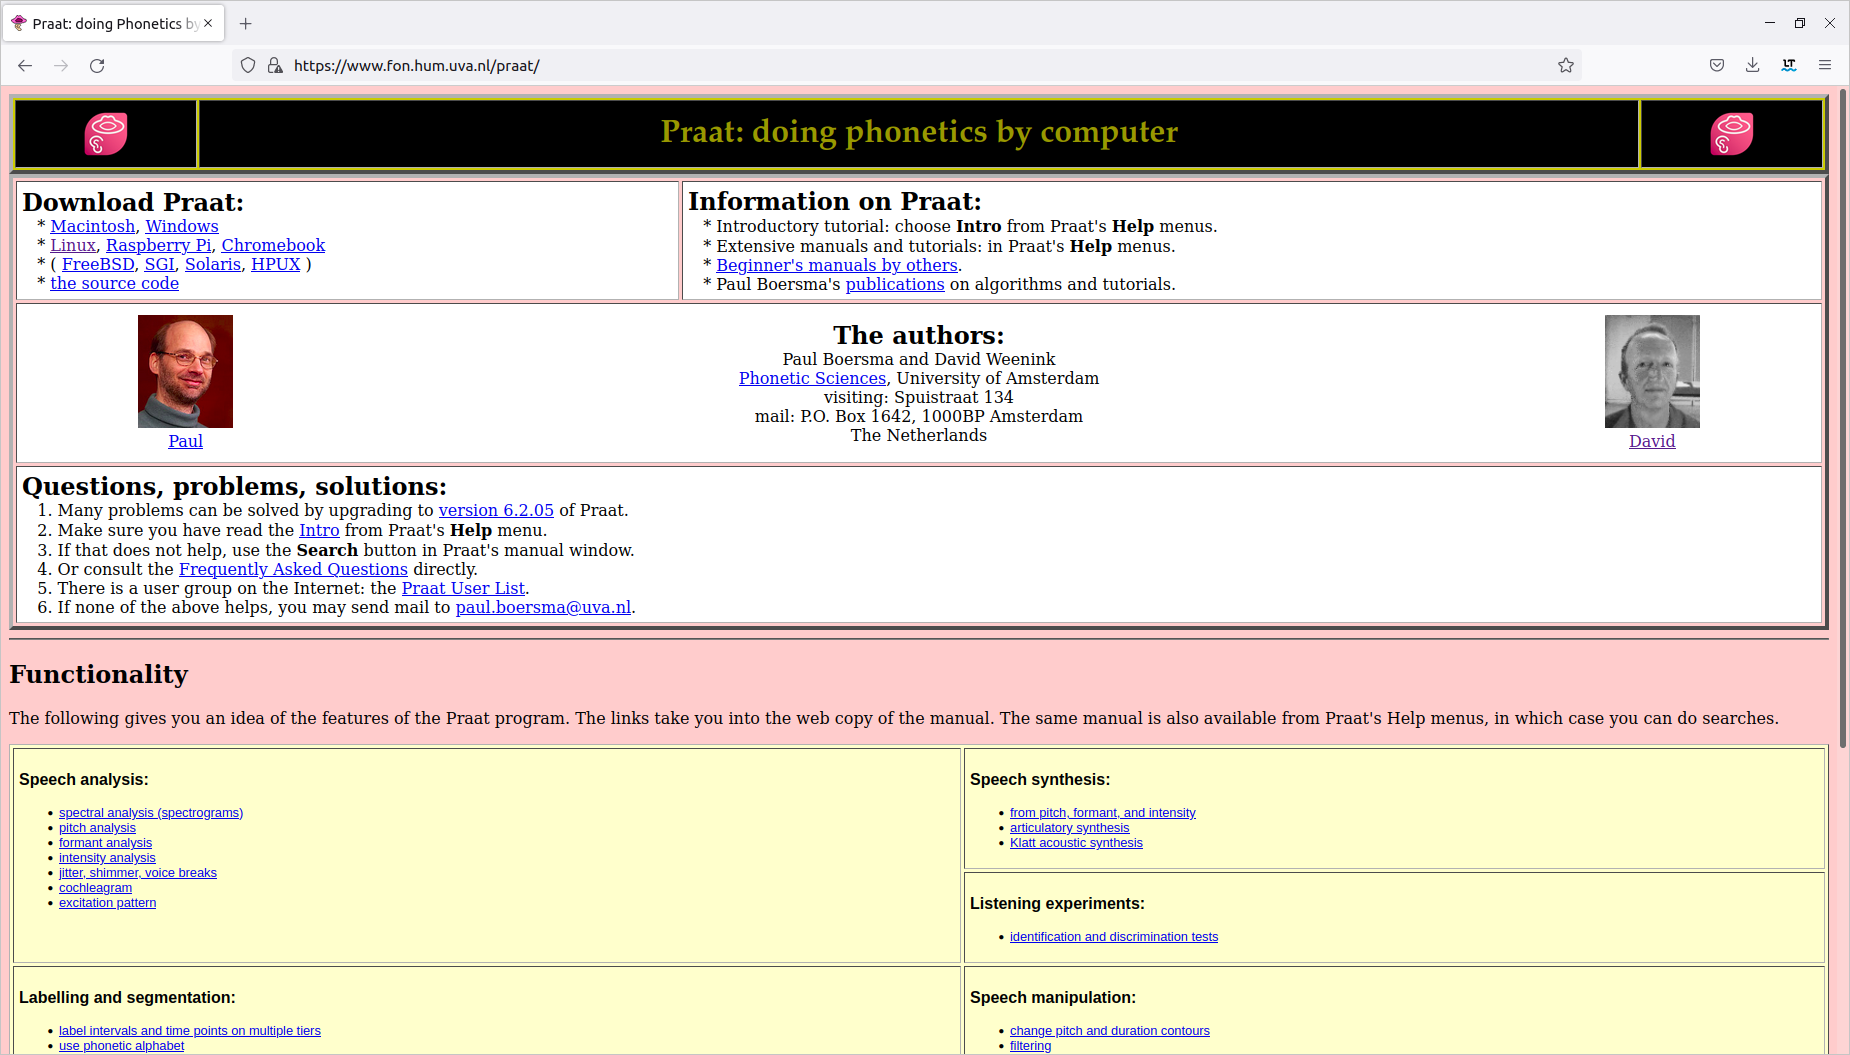
\includegraphics[width=1\textwidth]{Fig1.png}
 \caption{Página inicial do Praat.}
 \label{fig1}
 \source{\hyperlink{https://www.fon.hum.uva.nl/praat/}{https://www.fon.hum.uva.nl/praat/}.}
\end{figure}
%%FIGURA 1 - Página inicial do Praat

Na nova página, é apresentada a versão mais atual do programa, junto de materiais de apoio para a instalação e utilização do Praat (tais como instruções de instalação, tutoriais para novos usuários, pacotes de caracteres do IPA e versões do Praat compatíveis com versões antigas do sistema operacional), como se pode observar na Figura \ref{fig2}, que ilustra as opções de \textit{download} para Windows da página do Praat. 

\begin{figure}[H]
    \centering
    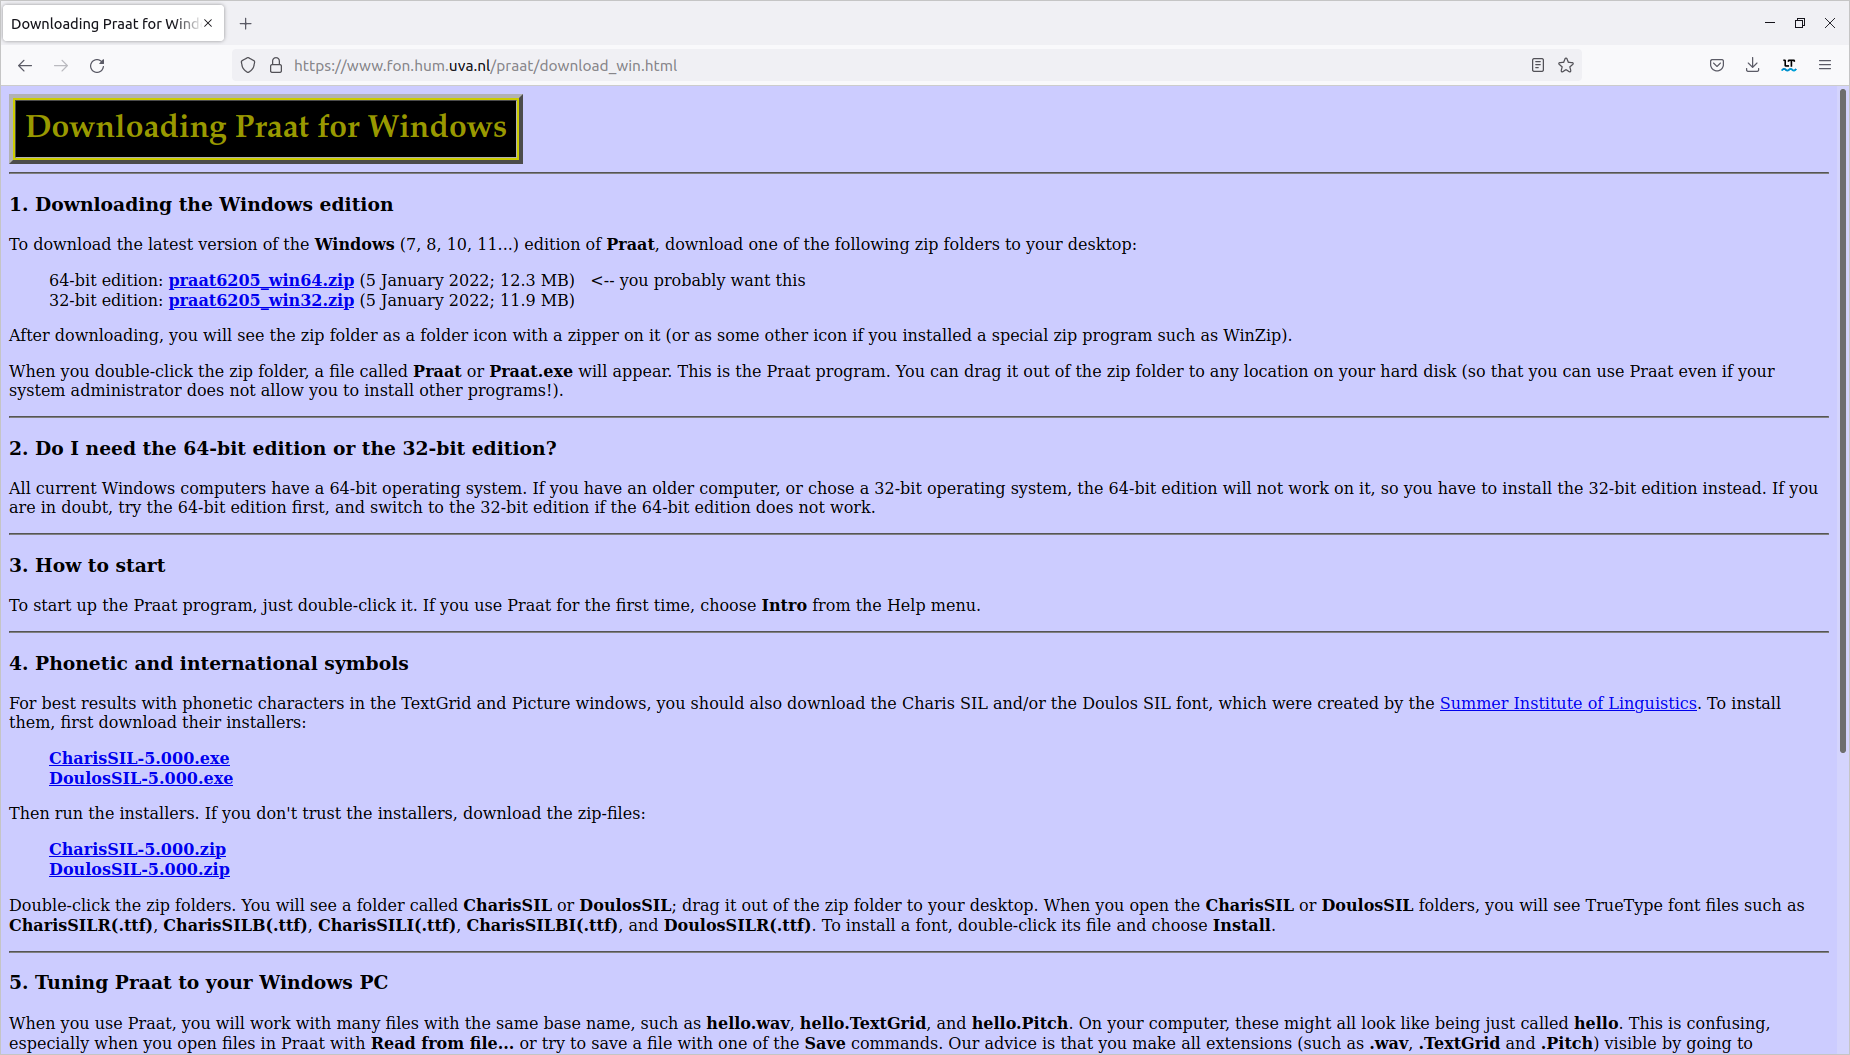
\includegraphics[width=1\textwidth]{Fig2.png}
    \caption{Página de \textit{download} do Praat para Windows.}
    \label{fig2}
    \source{ \hyperlink{https://www.fon.hum.uva.nl/praat/}{https://www.fon.hum.uva.nl/praat/}.}
\end{figure}
%%FIGURA 2 - Página de \textit{download} do Praat para Windows

Nesta tela, são disponibilizados os links para obter a edição de 64 ou 32 bits da versão mais atualizada do programa. O usuário da ferramenta deve selecionar a versão compatível com seu sistema operacional. Após fazer o \textit{download}, pode ser necessário extrair o programa do arquivo compactado (formato zip), o que pode ser feito pelos seguintes passos: clicar duas vezes sobre o arquivo baixado para abrir a pasta compactada, em seguida, clicar com o botão direito no arquivo ``Praat.exe'' e, por fim, selecionar ``Extrair para a pasta selecionada'' ou ``Extrair tudo''. Indique a pasta em que deseja extrair o Praat e clique em ``OK''. O programa poderá ser aberto a partir da pasta em que foi extraído, clicando sobre o seu ícone, ou por meio de um comando de execução. Em outros sistemas operacionais os procedimentos são análogos, portanto, não serão abordados neste texto.

\subsection{Primeiros passos}\label{sec-primeiros}
Após a inicialização do programa, duas janelas são abertas, a janela de objetos e a janela de imagens.A Figura \ref{fig3} mostra a janela de objetos, indicada por um retângulo azul, e a janela de figuras, indicada por um retângulo vermelho. A operação do Praat se concentra na utilização da janela de objetos, já que a partir dela é possível manipular, modificar, editar, anotar e analisar um arquivo de som e os diferentes tipos de objetos que podem ser gerados pelo programa. A janela de imagens tem uso mais específico: é usada para gerar figuras, frequentemente a partir de representações gráficas da fala. Além dessas duas janelas iniciais, outras janelas são abertas, à medida que as funções do programa são acionadas.

\begin{figure}[H]
 \centering
 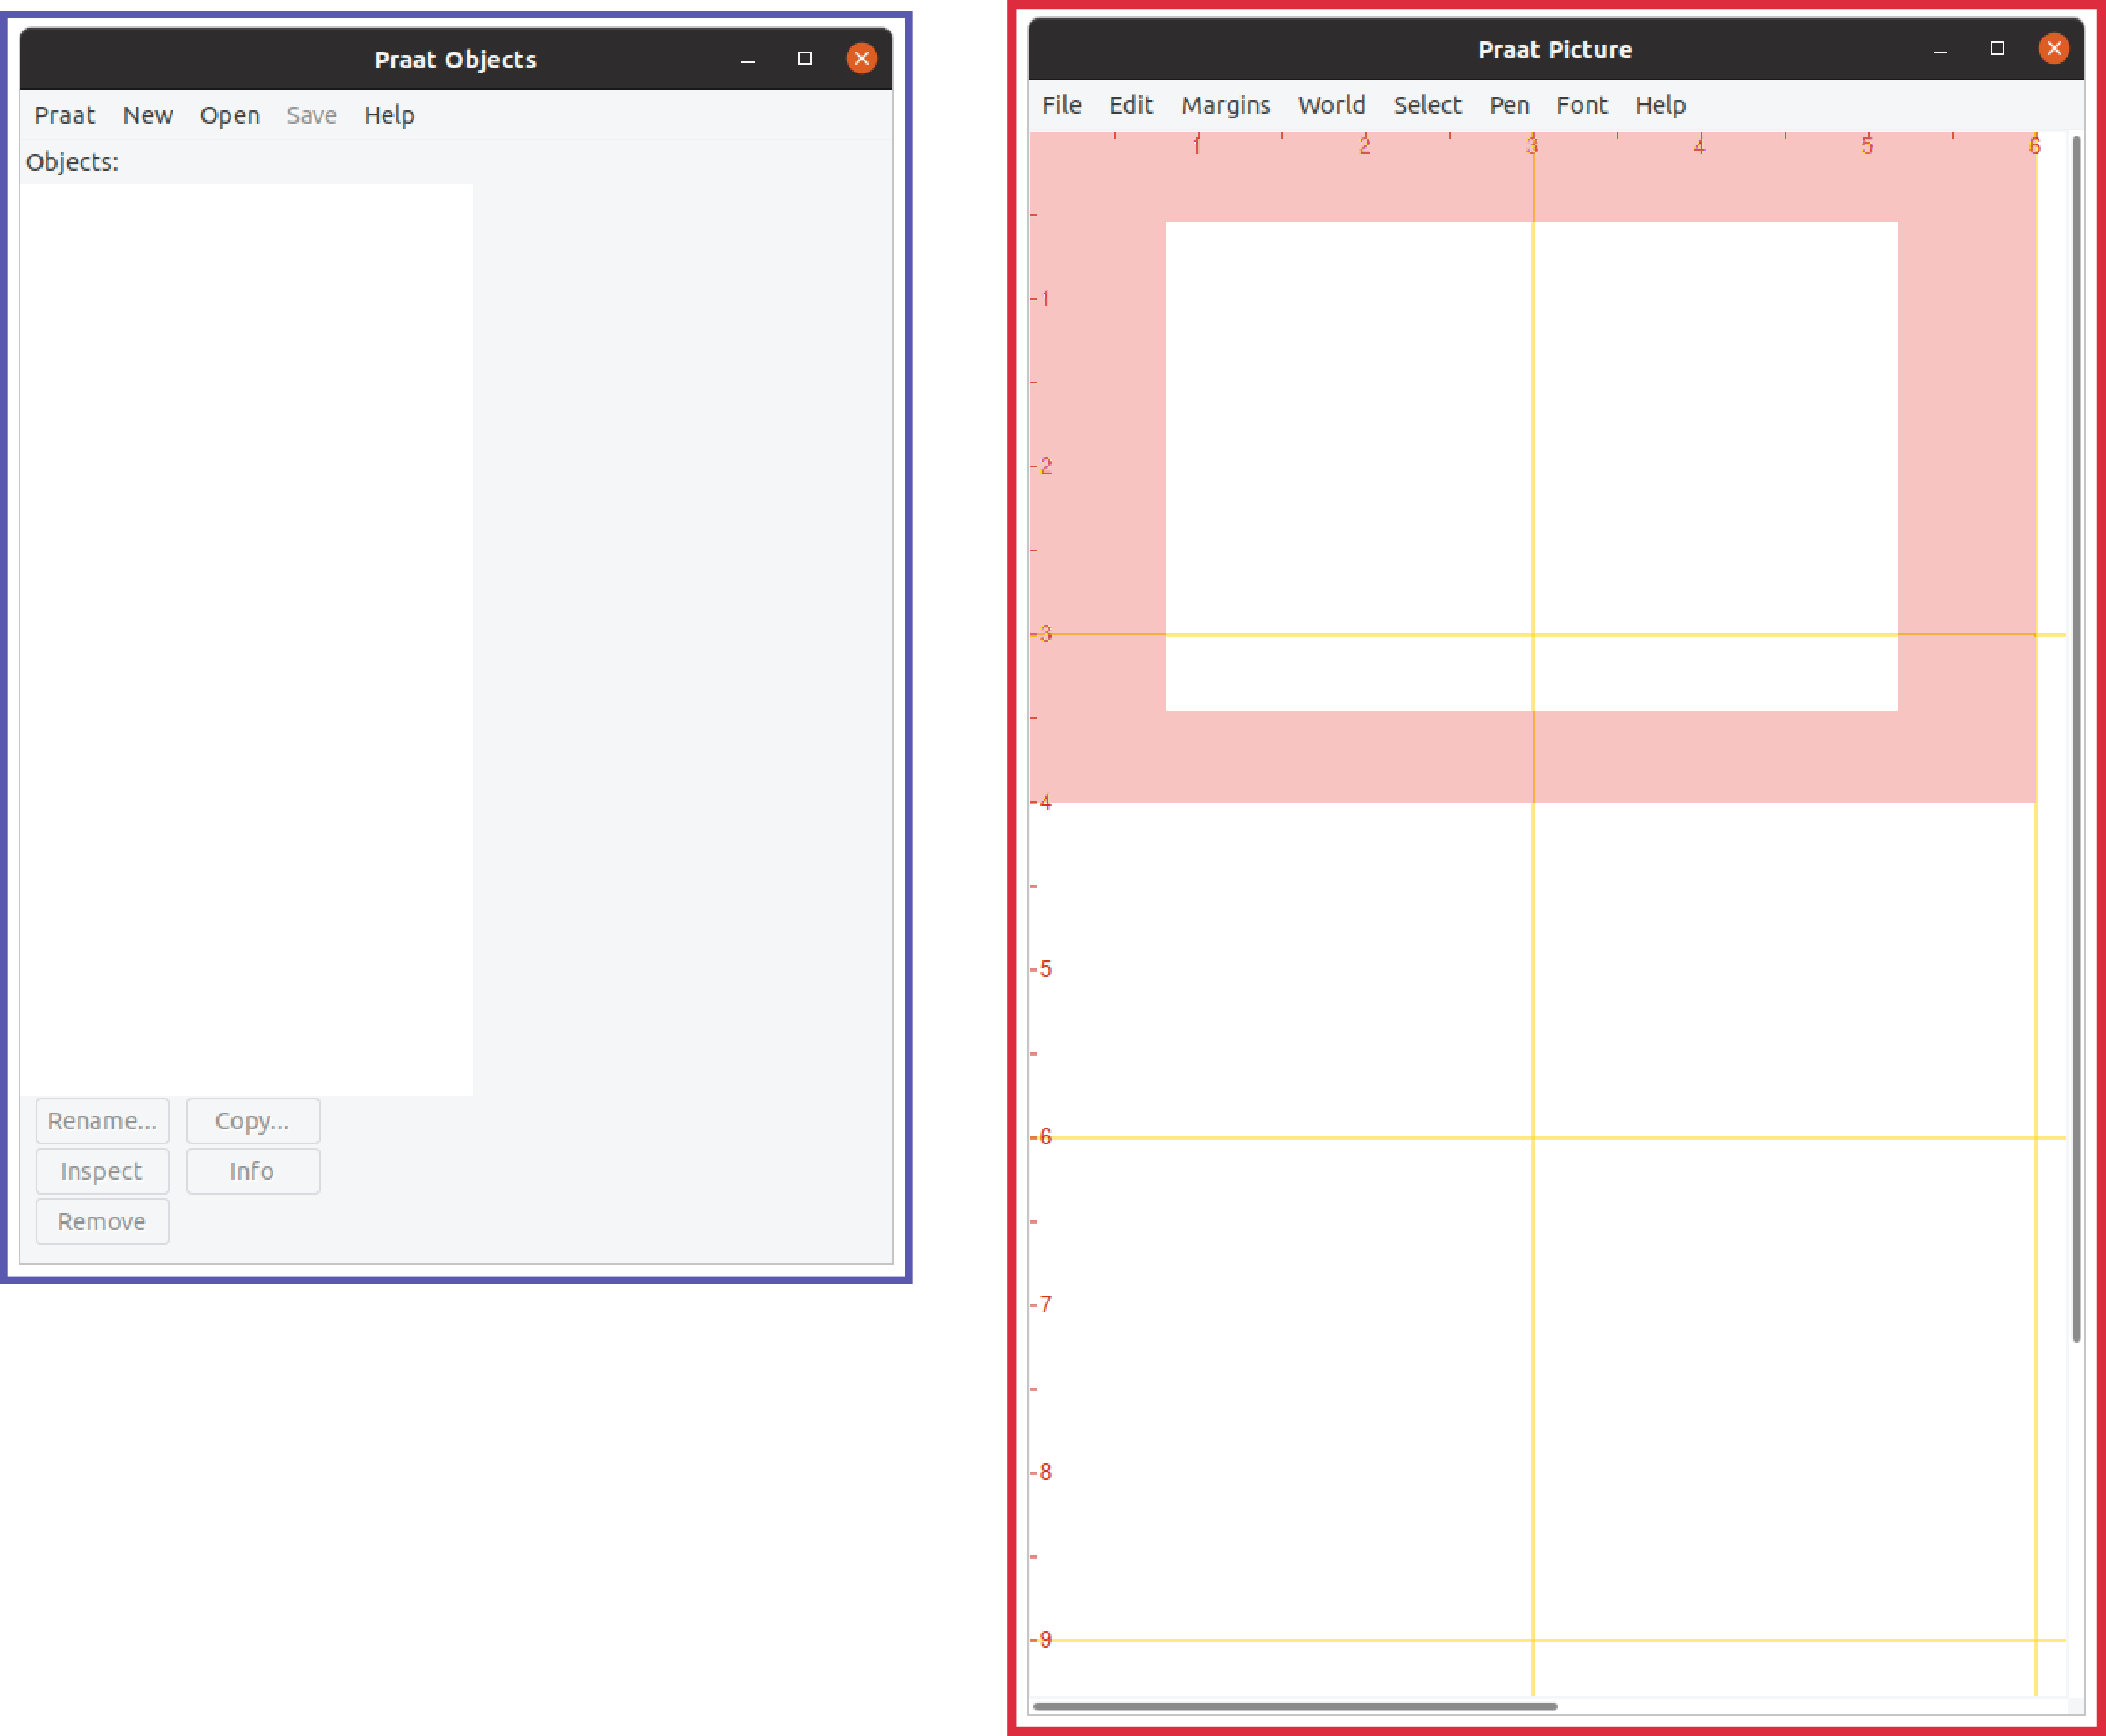
\includegraphics[width=1.0\textwidth]{Fig3.png}
 \caption{Janelas iniciais do Praat: a janela de objetos, indicada por um retângulo azul, e a janela de figuras, indicada por um retângulo vermelho.}
 \label{fig3}
 \source{Praat \cite{boersma_2022}.}
\end{figure}
%%FIGURA 3 - Janelas iniciais do Praat: a janela de objetos e a janela de figuras

A janela de objetos contém, no formato de uma lista, os diferentes elementos utilizados na análise. Frequentemente esses elementos são objetos de áudio, mas podem ser também objetos de anotação (TextGrid), objetos gráficos e diversos outros. Quando um objeto é selecionado na lista de objetos, uma série de opções específicas, relevantes para aquele objeto, surge à esquerda, nos botões do menu dinâmico.
  

\section{Geração e avaliação gráfica de ondas sonoras}\label{sec-intro-acustica}
Esta seção pretende apresentar alguns tipos elementares de ondas sonoras e como podem ser geradas e avaliadas graficamente, com o programa Praat. Os conceitos relacionados a ondas sonoras e sua representação gráfica apresentados na seção são classicamente usados na análise fonética desde os primeiros trabalhos de fonética acústica (e.g. o capítulo sobre fonética acústica na primeira edição de ``A Course in Phonetics'', por \textcite{ladefoged1975}). Para aprofundamento em análise acústica da fala, recomendamos a leitura de algum dos excelentes manuais disponíveis em português, como \textcite{cristofaro_etal_2019}, \textcite{barbosa_madureira_2015} ou \textcite{kent_read}, ou ainda, em inglês, \textcite{reetz_jongman_2011} ou \textcite{ladefoged_johnson_2014}.

\subsection{Ondas sonoras elementares}\label{sec-ondas}
O som é formado por perturbações das moléculas do ar capazes de ativar o sistema auditivo. Essas perturbações geram diferenças de pressão transmitidas espacialmente, na forma de ondas sonoras. Na fala, as ondas sonoras são produzidas pela movimentação de estruturas do aparelho fonador. 

As variações de pressão que geram as ondas sonoras são captadas, seja pelo ouvido humano, seja por um microfone, como oscilações que se estendem temporalmente. A magnitude das oscilações é definida como a \textbf{amplitude} da onda sonora. Por padrão, a amplitude, ou pressão sonora, é expressa em pascal (Pa), unidade do Sistema Internacional (SI), mas apenas em um áudio calibrado essa unidade é verdadeira. Em áudios sem calibração, a unidade de medida da amplitude é considerada arbitrária, mas ainda assim pode permitir avaliações da amplitude de sons da gravação, de forma relativa. A amplitude pode ainda ser escalonada, isto é, o valor de maior amplitude do arquivo de som pode ser alterado para um valor desejado e todos os outros valores de amplitude serão alterados proporcionalmente, sem distorcer o sinal. 

O intervalo de tempo em que ocorre um evento acústico é a sua \textbf{duração}, expressa em segundo (s) por padrão. Uma oscilação que se repete sistematicamente, com ciclos iguais, é periódica. A duração de um ciclo é chamada de \textbf{período} e sua taxa de repetição em um segundo é definida como sua \textbf{frequência}. Período (T) e frequência (F) se relacionam matematicamente por \(F = 1 / T\). Diferentes frequências estão associadas a diferentes oscilações presentes nas ondas sonoras. A frequência é expressa em hertz (Hz), que corresponde a ciclos por segundo. A Figura \ref{fig4} mostra a amplitude e o período de um tom simples, que é uma onda sonora composta por uma única frequência. 

\begin{figure}[htbp]
 \centering
 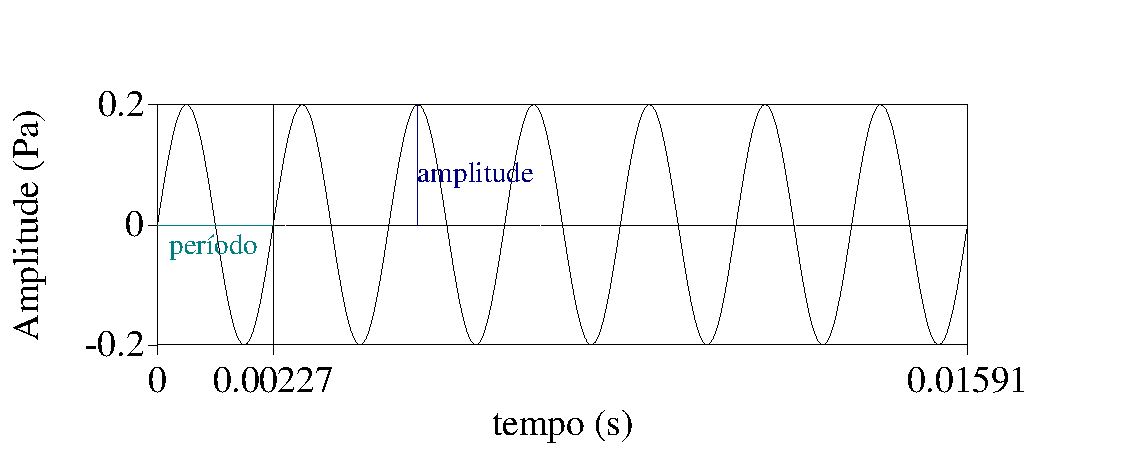
\includegraphics[width=0.7\textwidth]{Fig4.pdf}
 \caption{Propriedades elementares das ondas sonoras.}
 \label{fig4}
 \source{Elaboração própria.}
\end{figure}
%%FIGURA 4 - Propriedades elementares das ondas sonoras.

No exemplo de oscilação apresentado na Figura \ref{fig4}, a duração do intervalo mostrado é 0,016 s e há sete ciclos de repetição. A duração de um ciclo, ou período, é de 0,00227 s. A frequência é de aproximadamente 440 Hz (ou \(1 / 0,00227\) s). A amplitude é de 0,2 Pa. A Figura \ref{fig4} mostra um trecho de uma onda sonora gerada pelo Praat com a seguinte função: na janela de objetos, \textit{New $\rightarrow$ Sound $\rightarrow$  Create Sound from formula...} No parâmetro \textit{Name}, deve ser fornecido o nome desejado para o novo objeto. Em \textit{Number of channels}, use 1 para mono (ou 2 para estéreo). Os parâmetros em \textit{Start time} e \textit{End time} definem o intervalo temporal do objeto. Se \textit{Start time} é 0, \textit{End time} define a duração total. \textit{Sampling frequency} (taxa de amostragem) é o número de amostras contidas em cada segundo e corresponde ao dobro da maior frequência presente no objeto gerado. Para um objeto de áudio genérico, 44.100 Hz é geralmente usado, pois garante que as frequências audíveis estarão representadas. Em \textit{Formula} deve ser inserida uma expressão matemática que represente o sinal desejado. Na Figura \ref{fig4}, foi usada a seguinte expressão em \textit{Formula}, que gera um sinal senoidal com amplitude de 0,2 Pa e frequência de 440 Hz: \[1/5 \times sin(2 \times \pi \times 440 \times x)\].  

Um som semelhante pode ser gerado também a partir da função \textit{New $\rightarrow$ Sound $\rightarrow$  Create Sound as pure tone...}

As ondas da fala e a maioria dos sons cotidianos são caracterizadas por oscilações de amplitude em múltiplas frequências. As frequências da voz, assim como de certos instrumentos musicais e outros dispositivos, apresentam valores seguindo um padrão bem definido: formam uma série harmônica. A frequência mais baixa é chamada \textbf{frequência fundamental}, ou \textbf{F0}, que no caso da voz é determinada pela taxa de vibração das pregas vocais. Além de F0, estão presentes uma sequência de frequências com valores múltiplos inteiros da fundamental, chamados \textbf{harmônicos} (H1, H2, etc., sendo H1 a própria frequência fundamental). A Figura \ref{fig5} mostra dois exemplos: uma onda sonora periódica harmônica, com destaque para sua frequência fundamental e harmônicos, e uma onda sonora aperiódica, em que não há ciclos de repetição.

\begin{figure}[H]
 \centering
 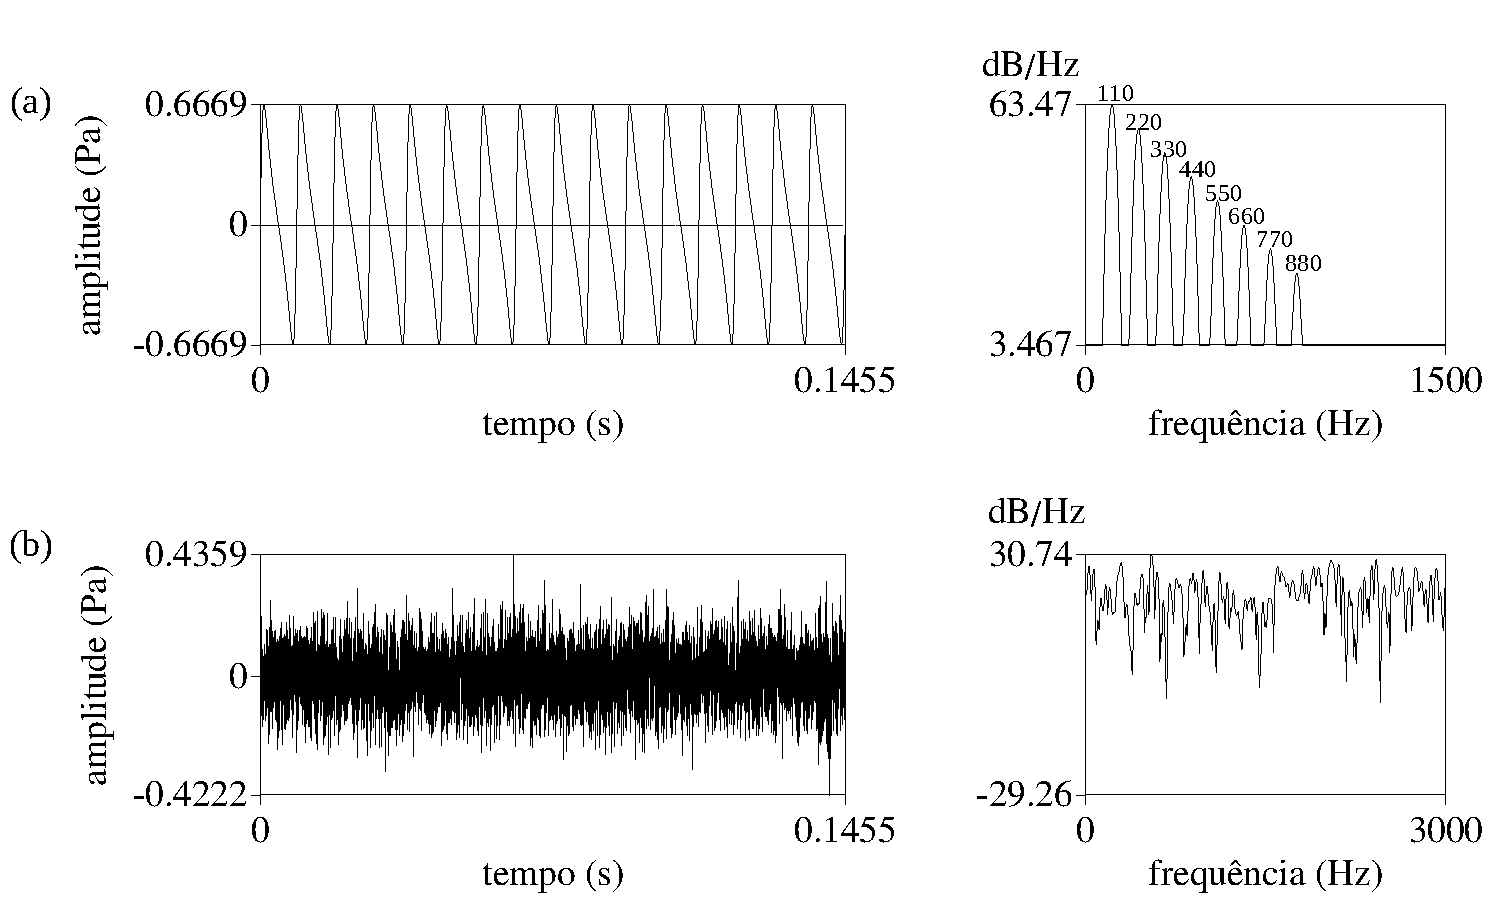
\includegraphics[width=0.9\textwidth]{Fig5.pdf}
 \caption{Exemplos de ondas sonoras: (a) periódica harmônica (oito primeiros harmônicos) e (b) aperiódica.}
 \label{fig5}
  \source{Elaboração própria.}
\end{figure}
%%FIGURA 5 - Exemplos de ondas sonoras: (a) periódica harmônica (oito primeiros harmônicos) e (b) aperiódica.

A Figura \ref{fig5}a mostra, à esquerda, uma onda sonora que contém oito frequências múltiplas inteiras. Esses harmônicos podem ser visualizados à direita como picos nas frequências de 110 Hz (H1 = F0), 220 Hz (H2), 330 Hz (H3), 440 Hz (H4) ... e 880 Hz (H8). A Figura \ref{fig5}a foi gerada no Praat com a mesma função e parâmetros da onda da Figura \ref{fig4}, usando em \textit{Formula} a seguinte expressão, que gera uma onda periódica complexa com oito componentes com as amplitudes e frequências especificados: 
\begin{align*}
1/2 \times sin(2 \times \pi \times 110 \times x) + 
1/4 \times sin(2 \times \pi \times 220\times x) + 
1/8 \times sin(2 \times \pi \times 330 \times x) \\ + 
1/16 \times sin(2 \times \pi \times 440 \times x) + 
1/32 \times sin(2 \times \pi \times 550\times x) + 
1/64 \times sin(2 \times \pi \times 660 \times x) \\ + 
1/128 \times sin(2 \times \pi \times 770 \times x) +
1/256 \times sin(2 \times \pi \times 880 \times x)
\end{align*}

A Figura \ref{fig5}b mostra, à esquerda, uma onda sonora aperiódica, em que não é possível identificar ciclos de repetição. À direita, em comparação com o mesmo gráfico da parte Figura \ref{fig5}a, vemos que não há picos bem definidos. A Figura \ref{fig5}b foi gerada no Praat com a mesma função e os mesmos parâmetros da onda \ref{fig5}a, usando em \textit{Formula} a seguinte expressão, que gera um ruído do tipo gaussiano, com média 0 e desvio padrão 0,1: \[randomGauss(0,0.1)\] 


\subsection{Representação gráfica do sinal da fala}\label{sec-representacao}
A representação gráfica das ondas sonoras é necessária para conferir aos estudos sobre a fala objetividade e precisão na análise dos dados. As três representações gráficas mais frequentemente utilizadas são definidas a seguir e ilustradas pela Figura \ref{fig6}.

A \textbf{forma de onda} (ou oscilograma) representa variações da pressão sonora ao longo do tempo. O \textbf{espectro} (ou espectro de amplitude) representa variações do nível de pressão sonora ao longo da frequência. Nesta representação, a dimensão do tempo não está presente. O \textbf{espectrograma} representa variações do nível de pressão sonora (escala de cinza) em diferentes frequências (eixo vertical) ao longo do tempo (eixo horizontal).

As Figuras \ref{fig6}a e \ref{fig6}b mostram respectivamente a forma de onda e o espectrograma de um trecho de áudio contendo a palavra ``festa''. A duração do trecho é de 0,5403 s. A forma de onda e o espectrograma estão alinhados temporalmente, de forma que compartilham o mesmo intervalo no eixo horizontal (tempo). A amplitude do trecho de áudio foi escalonada para 0,99. As Figuras \ref{fig6}c e \ref{fig6}d mostram o espectro da vogal [\textipa{E}] e da consoante [s] da palavra ``festa'' mostrada nas Figuras \ref{fig6}a e \ref{fig6}b. 

\begin{figure}[H]
 \centering
 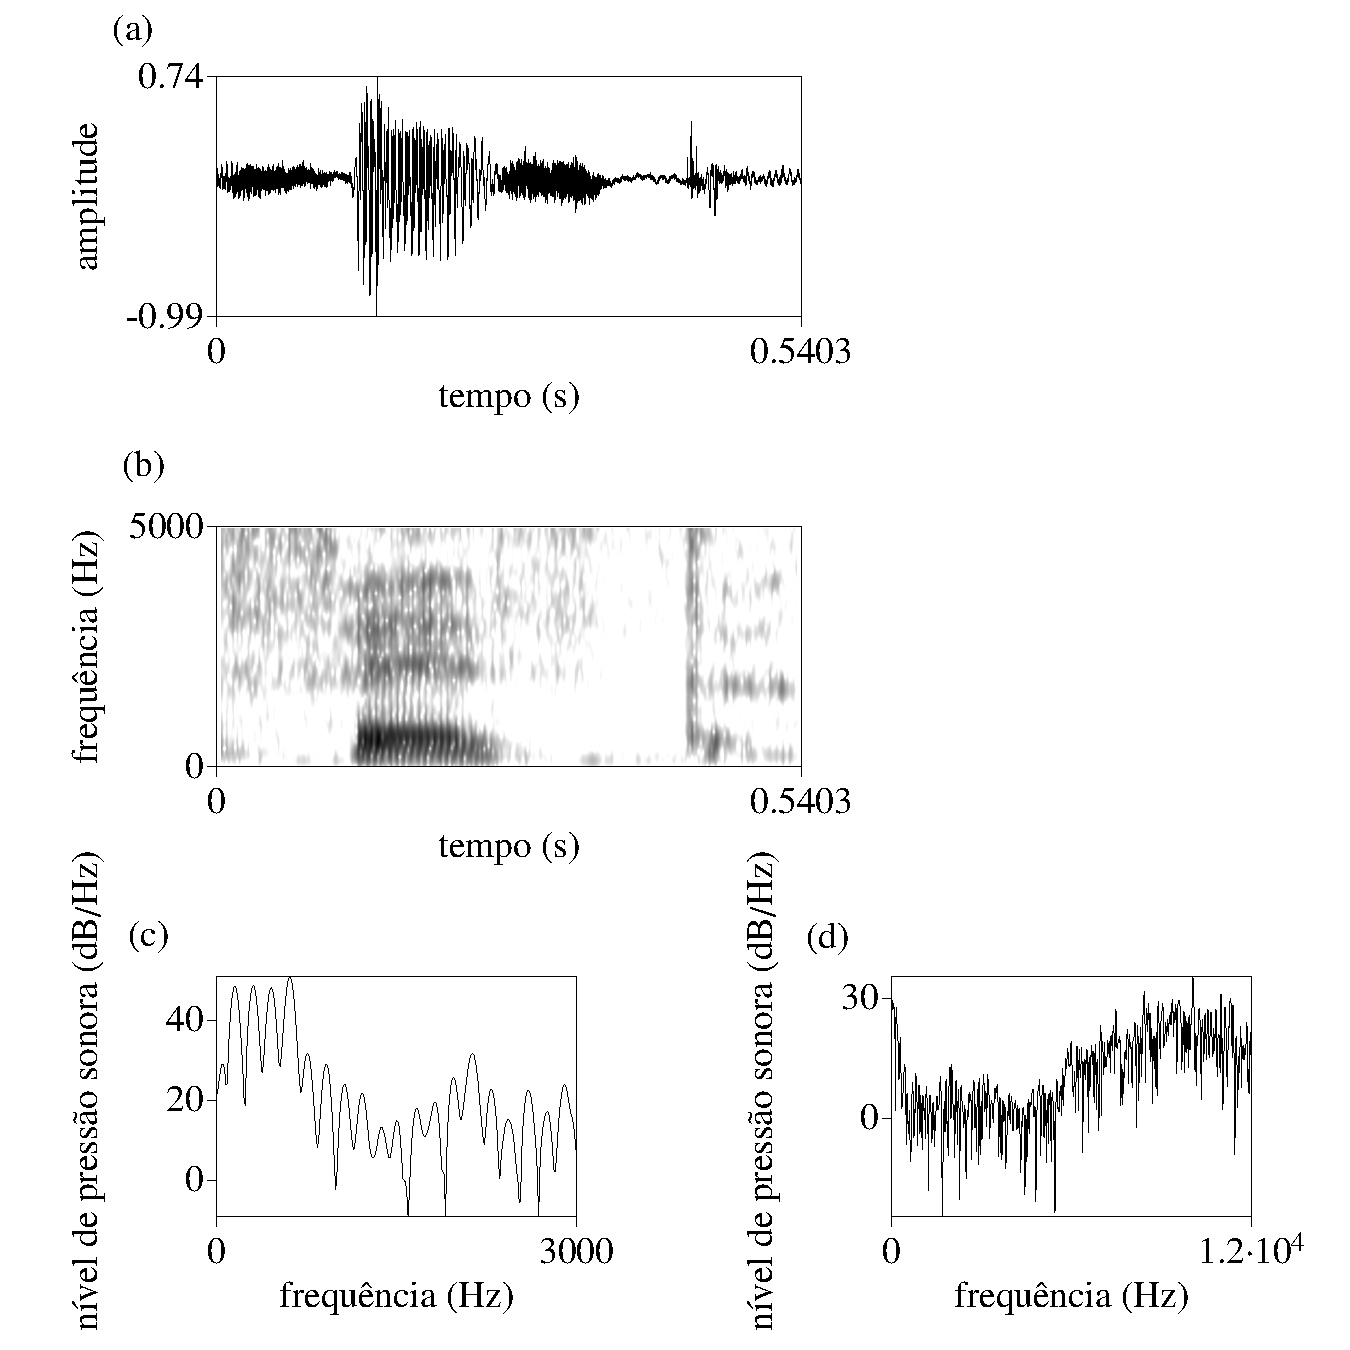
\includegraphics[width=0.9\textwidth]{Fig6.pdf}
 \caption{Representações gráficas usadas na análise fonética acústica: (a) forma de onda, (b) espectrograma, (c) espectro de uma vogal, (d) espectro de uma consoante.}
 \label{fig6}
 \source{Elaboração própria.}
\end{figure}
%%FIGURA 6 - Representações gráficas usadas na análise fonética acústica: (a) forma de onda, (b) espectrograma, (c) espectro de uma vogal, (d) espectro de uma consoante

Os áudios de fala utilizados na Figura \ref{fig6} e as demais imagens ilustrativas deste artigo foram selecionados a partir de listas de sentenças gravadas por um dos autores, uma falante nativa da variedade de Belo Horizonte, com nível superior de escolaridade e aos 35 anos. A gravação foi realizada na cabine acústica do Laboratório CEFALA, na Escola de Engenharia da UFMG, utilizando um gravador digital Micro Track II M-Audio e microfone Sennheiser HS 4 EW, em arquivo mono, 44.100 Hz e 16 bits.

\subsection{Operações básicas da análise acústica no Praat}\label{sec-operacoes} 
Uma ação frequente na análise acústica é a inspeção do sinal de áudio em análise, que pode ser realizada selecionando um objeto de som na janela de objetos e a opção \textit{View and edit}, no menu dinâmico à esquerda. Será aberta uma nova janela, a de visualização e edição, contendo a forma de onda (gráfico da parte superior e o espectrograma (gráfico da parte inferior), como mostra a Figura \ref{fig7}. 

\begin{figure}[H]
 \centering
 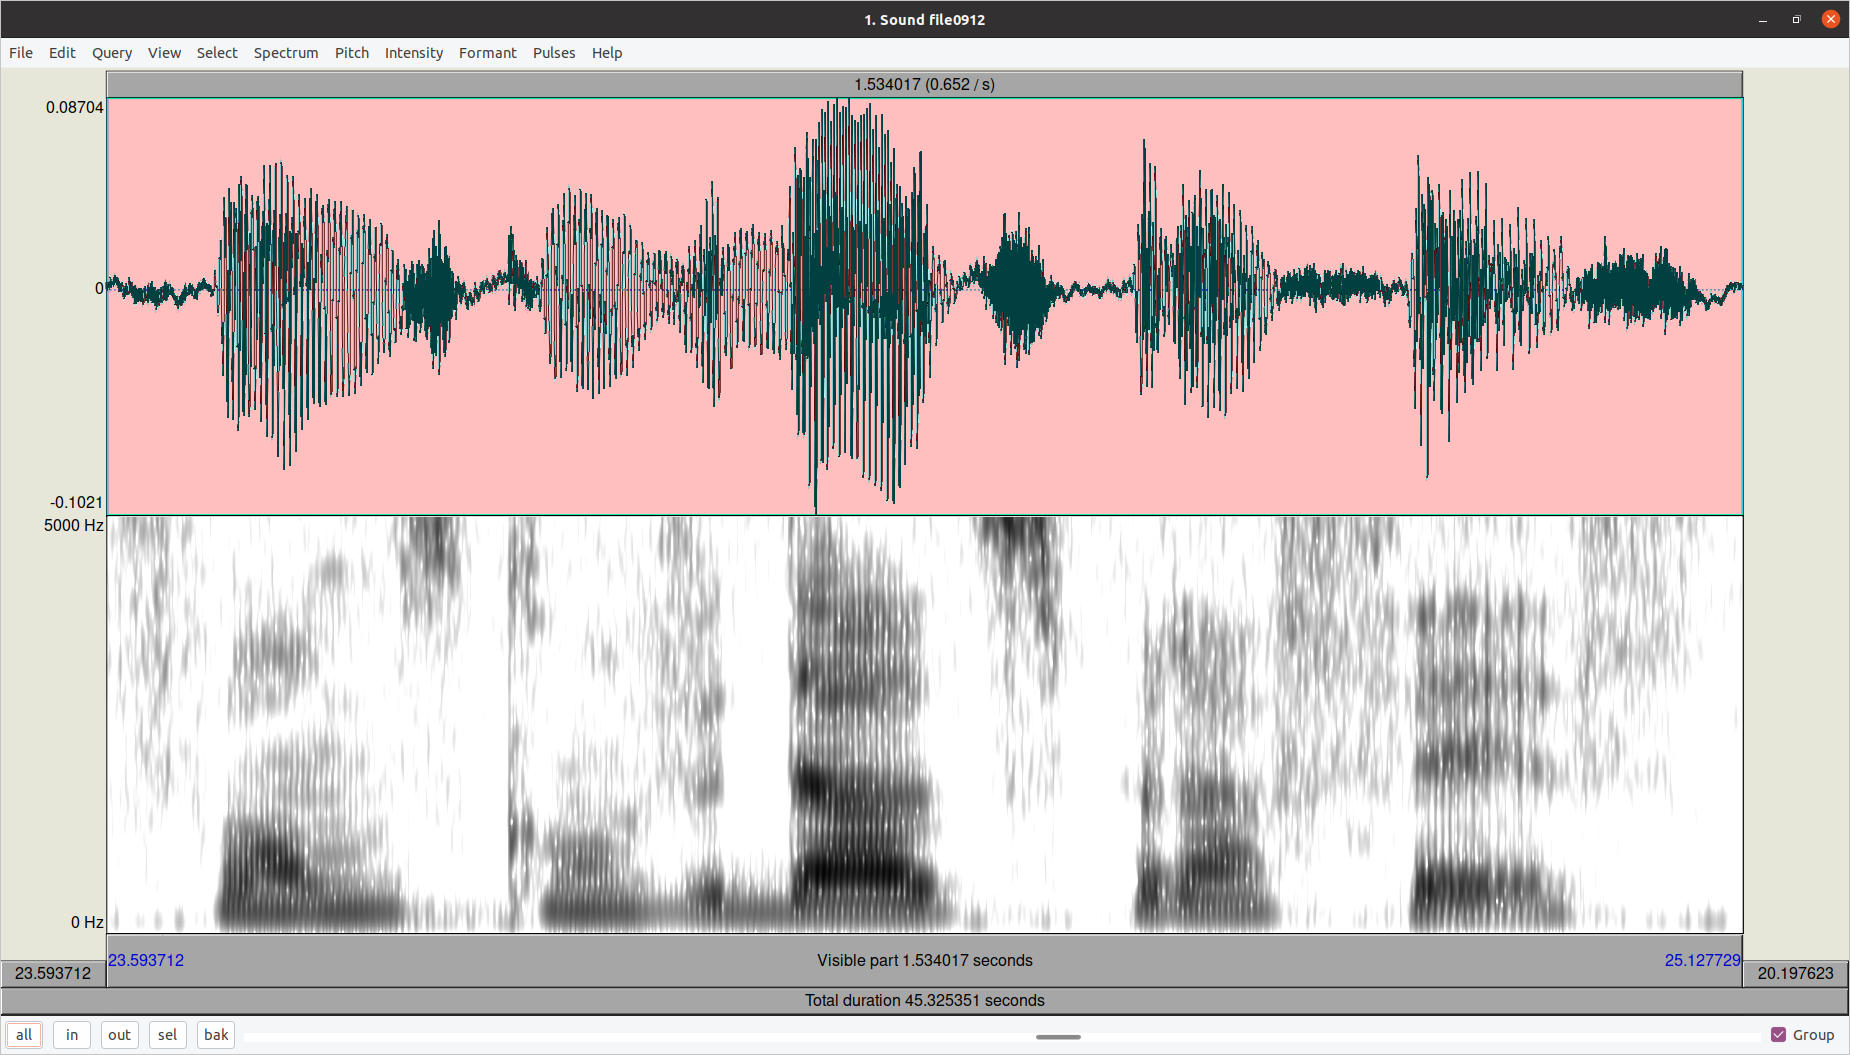
\includegraphics[width=0.7\textwidth]{Fig7.png}
 \caption{Janela de visualização e edição mostrando a forma de onda e o espectrograma de um áudio.}
 \label{fig7}
 \source{Praat \cite{boersma_2022}.}
\end{figure}
%%FIGURA 7 - Janela de visualização e edição mostrando a forma de onda e o espectrograma de um áudio

Na parte superior, há oito menus principais: \textit{file}, \textit{edit}, \textit{query}, \textit{view}, \textit{select}, \textit{spectrum}, \textit{pitch}, \textit{intensity}, \textit{formant}, \textit{pulse}. Ao clicar sobre cada um desses itens, abre-se uma listagem de comandos, ao lado dos quais podem estar especificados atalhos para acionamento pelo teclado.

O nível de zoom é controlado pelos comandos no menu \textit{View} ou pelos botões análogos na parte inferior, à esquerda: \textit{all} (zoom mínimo, visualiza todo o arquivo), \textit{in} (aumenta um nível de zoom), \textit{out} (diminui um nível de zoom), \textit{sel} (aplica o zoom exatamente à seleção atual), \textit{bak} (retorna para o nível anterior). O uso de atalhos, mostrados na Figura \ref{fig8}, facilita as transições entre diferentes níveis de zoom.

\begin{figure}[H]
 \centering
 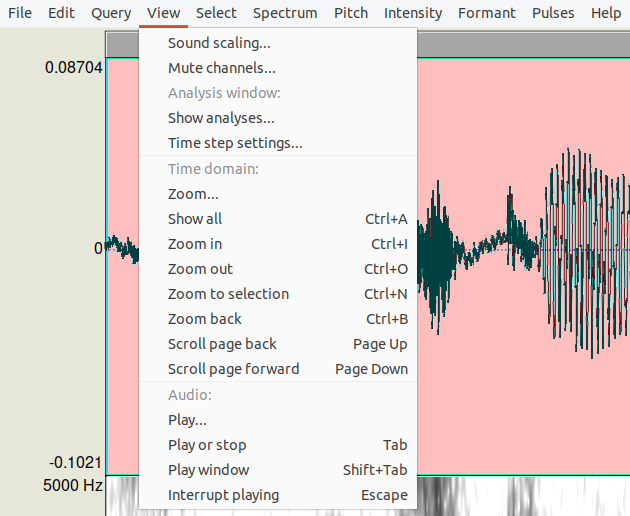
\includegraphics[width=0.6\textwidth]{Fig8.png}
 \caption{Menu \textit{View} expandido, mostrando os atalhos pertinentes.}
 \label{fig8}
  \source{Praat \cite{boersma_2022}.}
\end{figure}
%%FIGURA 8 - Menu \textit{View} expandido, mostrando os atalhos pertinentes

Algumas informações numéricas relativas aos eixos dos gráficos são apresentadas por padrão, como a duração total do arquivo, abaixo do espectrograma, a duração da seleção, no topo da forma de onda. Para tocar o arquivo de áudio, basta clicar sobre a barra que mostra a duração da seleção, acima da forma de onda, ou usar o atalho ``Tab''.

Ao lidar com arquivos de áudio na análise da fala, outros recursos básicos de processamento são frequentemente necessários. A seguir apresentaremos alguns recursos para objeto de áudio, de acordo com sua localização na janela de objetos. 

\hfill \break
\\Recursos acessados pelo menu superior da janela de objetos:
\begin{itemize}
\item Abrir um arquivo de som do computador: \textit{Read from file} (ou \textit{Open long sound file}, se o arquivo for extenso, por exemplo, muitos minutos ou horas de gravação; nesse modo de abertura, algumas funções são desabilitadas para evitar a sobrecarga da memória do programa). 
\item Gravar um som novo: \textit{New $\rightarrow$ Record mono sound} (abre interface para gravar áudio com um canal) \textit{$\rightarrow$ Record} (pode ser mantida a taxa de amostragem de 44.100 Hz comumente usada para a fala) \textit{$\rightarrow$ Stop} (quando terminar de gravar) \textit{$\rightarrow$ Save to list} (Será gerado um novo objeto na janela de objetos). \textbf{Atenção:} Para que seja armazenado permanentemente no computador, deve ser salvo como \textit{Save $\rightarrow$ Save as WAV file}.
\item Conseguir ajuda sobre um recurso e consultar o manual: \textit{Help}.
\end{itemize}

\hfill \break
\\Recursos acessados pelo menu dinâmico da janela de objetos:
\begin{itemize}
\item Obter taxa de amostragem: \textit{Query $\rightarrow$ Query time sampling $\rightarrow$ Get sampling frequency}.
\item Alterar a taxa de amostragem, ou seja, reamostrar: \textit{Convert $\rightarrow$ Resample} (Em \textit{New frequency rate}, informar a nova frequência de amostragem desejada, preferencialmente submúltipla da original. Em \textit{Precision rate}, manter o valor padrão de 50. Será gerado um novo objeto na janela de objetos).
\item Extrair um canal de um arquivo estéreo: \textit{Convert $\rightarrow$ Extract one channel} (escolher o número do canal que será mantido. Será gerado um novo objeto na janela de objetos)
\item Fundir (mixar) dois canais de um arquivo estéreo: \textit{Combine $\rightarrow$ Combine to stereo} (Será gerado um novo objeto de som com dois canais na janela de objetos).
\item Escalonar amplitude: \textit{Modify $\rightarrow$ Scale peak} (usar o valor desejado ou o padrão 0,99, que otimiza a audibilidade do áudio, sendo este o maior valor de amplitude que pode ser tocado sem distorção).
\end{itemize}

\section{Segmentação e anotação}\label{sec-segmentacao}
A segmentação da fala, no contexto da análise fonética acústica, consiste na delimitação de um trecho de fala em eventos sonoros de interesse (consoantes, vogais, sílabas etc.). Nesta seção, trataremos criticamente da segmentação da fala, bem como apresentaremos a tarefa de anotação e como esta pode ser realizada no Praat.
 
A análise fonética, assim como a fonológica, se baseia no princípio de que é possível decompor um enunciado falado em unidades discretas, como consoantes e vogais. Ressalte-se, contudo, que a fala é produzida pelas estruturas do trato vocal, que se movem continuamente e gradualmente ao longo do tempo. É notável que os diferentes sons que compõem sílabas, palavras e sentenças se sucedem sem que haja necessariamente uma interrupção ou descontinuidade entre eles. Ou, quando há descontinuidades, nem sempre correspondem ao que concebemos como as fronteiras entre os segmentos. Além disso, os sons sucessivos interferem uns nos outros e suas diferentes combinações geram diferentes padrões de transição, coarticulação e alterações sonoras. Observe na Figura \ref{fig9}, que corresponde à produção da sequência de palavras  ``durante séculos''. 

\begin{figure}[htbp]
 \centering
 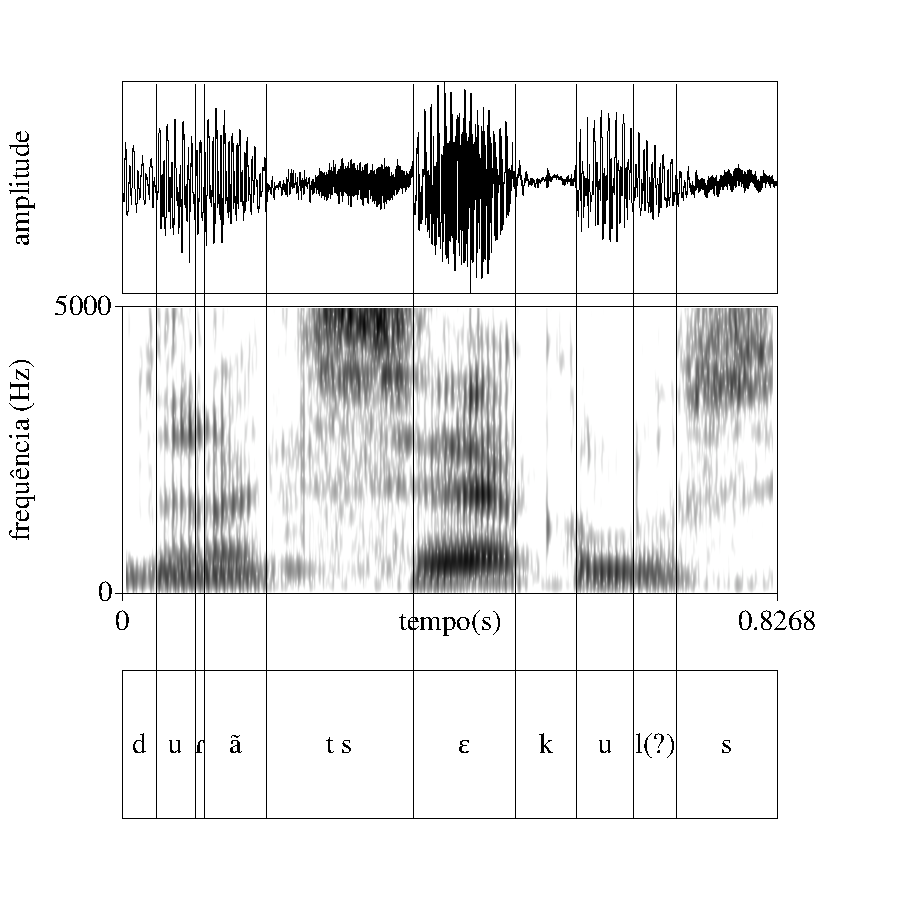
\includegraphics[width=0.7\textwidth]{Fig9.pdf}
 \caption{Forma de onda e espectrograma representando a continuidade fonética.}
 \label{fig9}
 \source{Elaboração própria.}
\end{figure}
%%FIGURA 9 - Forma de onda e espectrograma representando a continuidade fonética

No trecho mostrado na Figura \ref{fig9}, a vogal final de ``durante'' não foi pronunciada e a africada da última sílaba se funde com a fricativa no início da palavra ``século'', por sua similaridade fonética. A tarefa de separar a africada e a fricativa é complicada.

Outro desafio na tarefa de segmentação da fala é a dificuldade de se encontrar aspectos estritamente constantes que possam ser usados para definição de fronteiras. Essa dificuldade decorre da alta variabilidade dos sons da fala, atestada na produção de um mesmo falante, ainda mais evidente nas produções de diferentes falantes e afetada por fatores relacionados ao contexto de produção do enunciado. Para minimizar os problemas levantados acima, a segmentação da fala deve ser realizada a partir de \textbf{critérios de segmentação}, que devem ser fundamentados teoricamente, bem delimitados e seguidos de forma sistemática para todos os dados avaliados no estudo. De preferência, devem ser os mesmos critérios amplamente empregados em outros estudos, para permitir a compatibilidade dos resultados. Se possível, escolha sons e contextos que propiciem uma segmentação precisa. 

A \textbf{anotação}, no contexto da análise acústica, é a atribuição de informações a trechos da onda sonora. Entre as suas principais finalidades estão a identificação de eventos de interesse no sinal de áudio, o armazenamento de intervalos ou pontos usados para análises e medições, para acesso posterior (memória de análise), e a automatização de medidas (via \textit{scripts}). 

No Praat, as tarefas de segmentação e anotação são realizadas por meio de um recurso chamado TextGrid, ou grade textual, que consiste em um objeto de texto alinhado temporalmente com arquivo de som. Esse objeto de texto pode ser aberto juntamente com o arquivo de áudio correspondente, gerando opções adicionais na janela de visualização e edição. Nessa janela, camadas (\textit{tiers}) são usadas para separar diferentes tipos de eventos observados. As camadas podem ser determinadas pelo usuário em quantidade, tipo (um ponto ou um intervalo), posição e nome. Nas camadas são inseridas fronteiras (\textit{boundaries}), que representam o início e o fim dos eventos segmentados, no caso de uma camada de intervalo, ou representam o próprio evento, no caso de uma camada pontual. O tipo de camada é determinado ao gerar o objeto TextGrid e novas camadas, de qualquer um dos tipos, podem ser adicionadas posteriormente. 

Um arquivo TextGrid é gerado pelos seguintes passos: na janela de objetos, selecione um arquivo de áudio. No menu dinâmico, selecione o botão \textit{Annotate} e então \textit{To TextGrid}. Na janela de opções, em \textit{All tier names}, insira os nomes de cada uma das camadas que deseja inserir no TextGrid. Em \textit{Which of these are point tiers?}, especifique qual das camadas mencionadas no campo anterior é do tipo pontual. Se todas forem de intervalo, deixe este último campo vazio. Será gerado um novo objeto, de tipo TextGrid, na janela de objetos, com o mesmo nome do arquivo de áudio. É recomendado manter os nomes do TextGrid e do áudio iguais, a menos que haja uma razão específica para diferenciá-los. Selecione o objeto TextGrid junto com o áudio, apertando ``Ctrl'' no teclado, e, no menu dinâmico, selecione \textit{View and Edit}. A nova janela que será mostrada é semelhante à janela de visualização e edição, exceto pela presença das camadas criadas, na parte inferior da janela, como mostra a Figura \ref{fig10}.

\begin{figure}[H]
 \centering
 
\includegraphics[width=0.9\textwidth]{Fig10.png}
 \caption{Janela de visualização e edição acrescida das camadas de um arquivo TextGrid.}
 \label{fig10}
  \source{Praat \cite{boersma_2022}.}
\end{figure}
%%FIGURA 10 - Janela de visualização e edição acrescida das camadas de um arquivo TextGrid

É possível usar símbolos fonéticos do IPA para realizar as anotações em um TextGrid. Trata-se de uma opção interessante para utilização em trabalhos e publicações, com finalidade estética e interpretativa. Fora desse contexto de aplicação, é melhor usar caracteres comuns, para evitar problemas de codificação de caracteres (e possível perda de informações) e comprometimento do uso de \textit{scripts}. Pode ser mostrada na janela de edição do TextGrid um painel com símbolos do IPA, para facilitar sua inserção aos rótulos, com um clique. Esse recurso pode ser habilitado e desabilitado em \textit{File $\rightarrow$ Preferences $\rightarrow$ Show IPA chart}. A Figura \ref{fig11} mostra a janela de visualização após a habilitação do painel de fontes fonéticas.

\begin{figure}[H]
 \centering
 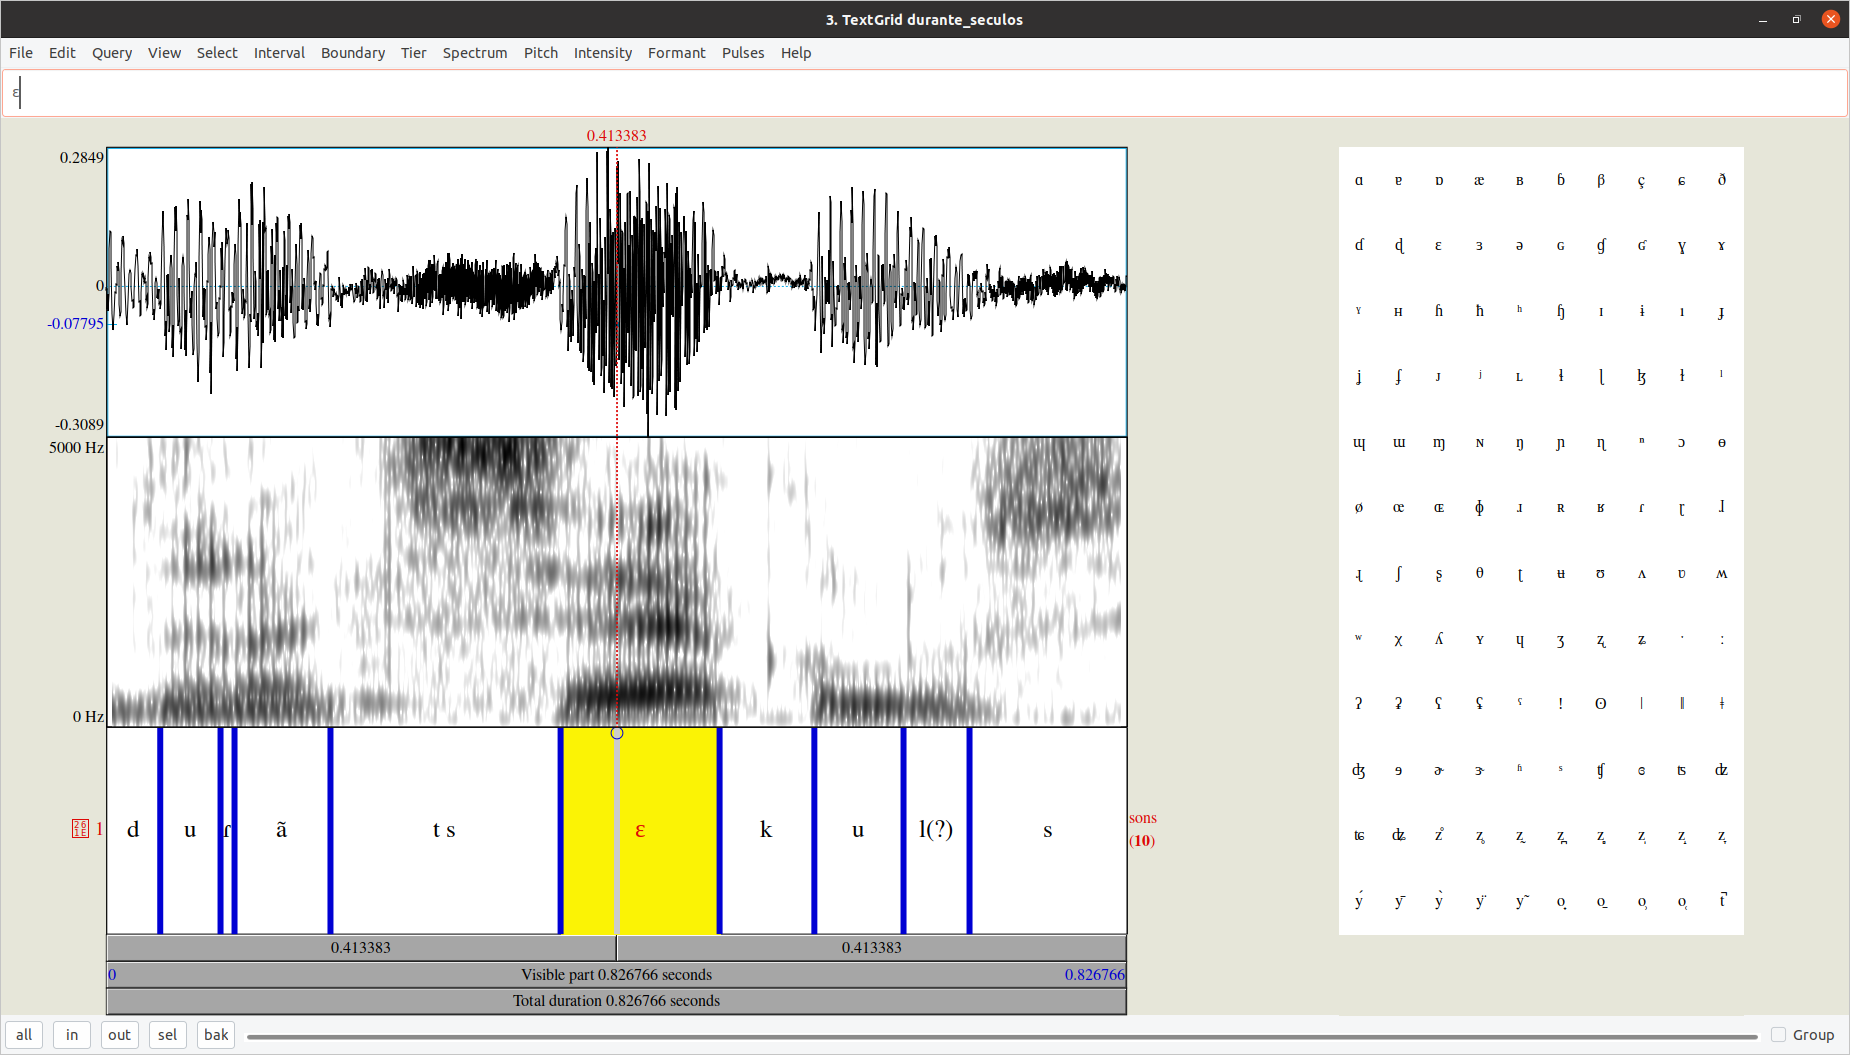
\includegraphics[width=0.9\textwidth]{Fig11.png}
 \caption{Janela de visualização e edição de áudio e TextGrid, com painel de fontes fonéticas.}
 \label{fig11}
  \source{Praat \cite{boersma_2022}.}
\end{figure}
%%FIGURA 11 - Janela de visualização e edição de áudio e TextGrid, com painel de fontes fonéticas

Outra forma de utilizar símbolos fonéticos no TextGrid é por meio de sequências de três caracteres (trígrafos) iniciada por uma barra inclinada para a esquerda (também chamada no Praat de \textit{backslash sequence} ou \textit{backslash trigraphs}), que podem ser interpretadas como símbolos do IPA, entre outras possibilidades. Por exemplo: $\backslash$ef para \textipa{E} ou $\backslash$sh para \textesh. Esse recurso permite também a representação de outros símbolos especiais, como símbolos matemáticos e letras gregas. É possível transpor o sistema de representação por trígrafos para símbolos do IPA mudando a codificação de caracteres do arquivo TextGrid para Unicode: após abrir o arquivo TextGrid, com ou sem o áudio, escolha \textit{Edit $\rightarrow$ Convert entire TextGrid to Unicode}. O procedimento inverso também é possível e pode ser realizado por  \textit{Edit $\rightarrow$ Convert entire TextGrid to backslash trigraphs}. A ação de conversão pode ser visualizada na barra de entrada de texto, na parte superior da janela de edição do TextGrid, mas nos dois modos de representação símbolos fonéticos serão mostrados nos rótulos do TextGrid. Ao utilizar um \textit{script} para processar os TextGrids, deve-se converter os arquivos para o formato de trígrafos.

Uma lista das opções de trígrafos disponíveis pode ser encontrada em \textit{Help $\rightarrow$ Go to manual page} e digite \textit{Special Symbols}. Para um quadro com a correspondência entre trígrafos e símbolos fonéticos, acesse \textit{Help $\rightarrow$ Go to manual page} e digite \textit{Phonetic symbols}.

\section{Análise acústica das vogais}\label{sec-vogais}
Nesta seção, iremos apresentar algumas propriedades acústicas das vogais, associadas às suas características articulatórias, e métodos de medição mais frequentemente utilizados para avaliação acústica das vogais.

\subsection{Formantes}\label{sec-formantes}

A descrição articulatória das vogais se baseia na posição horizontal e vertical da língua durante sua produção. Com base na altura da língua, uma vogal pode ser alta, média ou baixa. Em português, utilizamos dois níveis de altura para vogais médias (médias-altas e médias-baixas). Com base no avanço ou recuo da língua, uma vogal pode ser anterior, central ou posterior. 

Na produção dos sons da fala, o trato vocal funciona como uma cavidade de ressonância, capaz de modificar as ondas sonoras produzidas pela fonação. As ressonâncias amplificam seletivamente o sinal acústico em regiões de frequência próximas às frequências de ressonância da cavidade, que, por sua vez, dependem da configuração articulatória do trato. Como consequência dessa amplificação seletiva surgem os \textbf{formantes}, que são ondulações no espectro dos sons da fala emitidos e que dependem diretamente das frequências de ressonância da cavidade. Formantes são eventos acústicos que podem ser sistematicamente associados à posição da língua durante a produção de uma vogal. Os formantes relevantes para a caracterização das vogais são os três primeiros (F1, F2 e F3), mas especialmente os dois primeiros estão relacionados à diferenciação das vogais em termos de altura e anterioridade. F1 está relacionado à altura da vogal: quanto mais alta a vogal, menor o valor de F1. F2 está relacionado à anterioridade/posterioridade da vogal: quanto mais anterior a vogal, maior o valor do F2. A Figura \ref{fig12} mostra espectrogramas das sete vogais orais tensas do português, com traçado dos formantes, e permite a avaliação de como os dois primeiros formantes se relacionam à qualidade das vogais.

\begin{figure}[H]
 \centering
 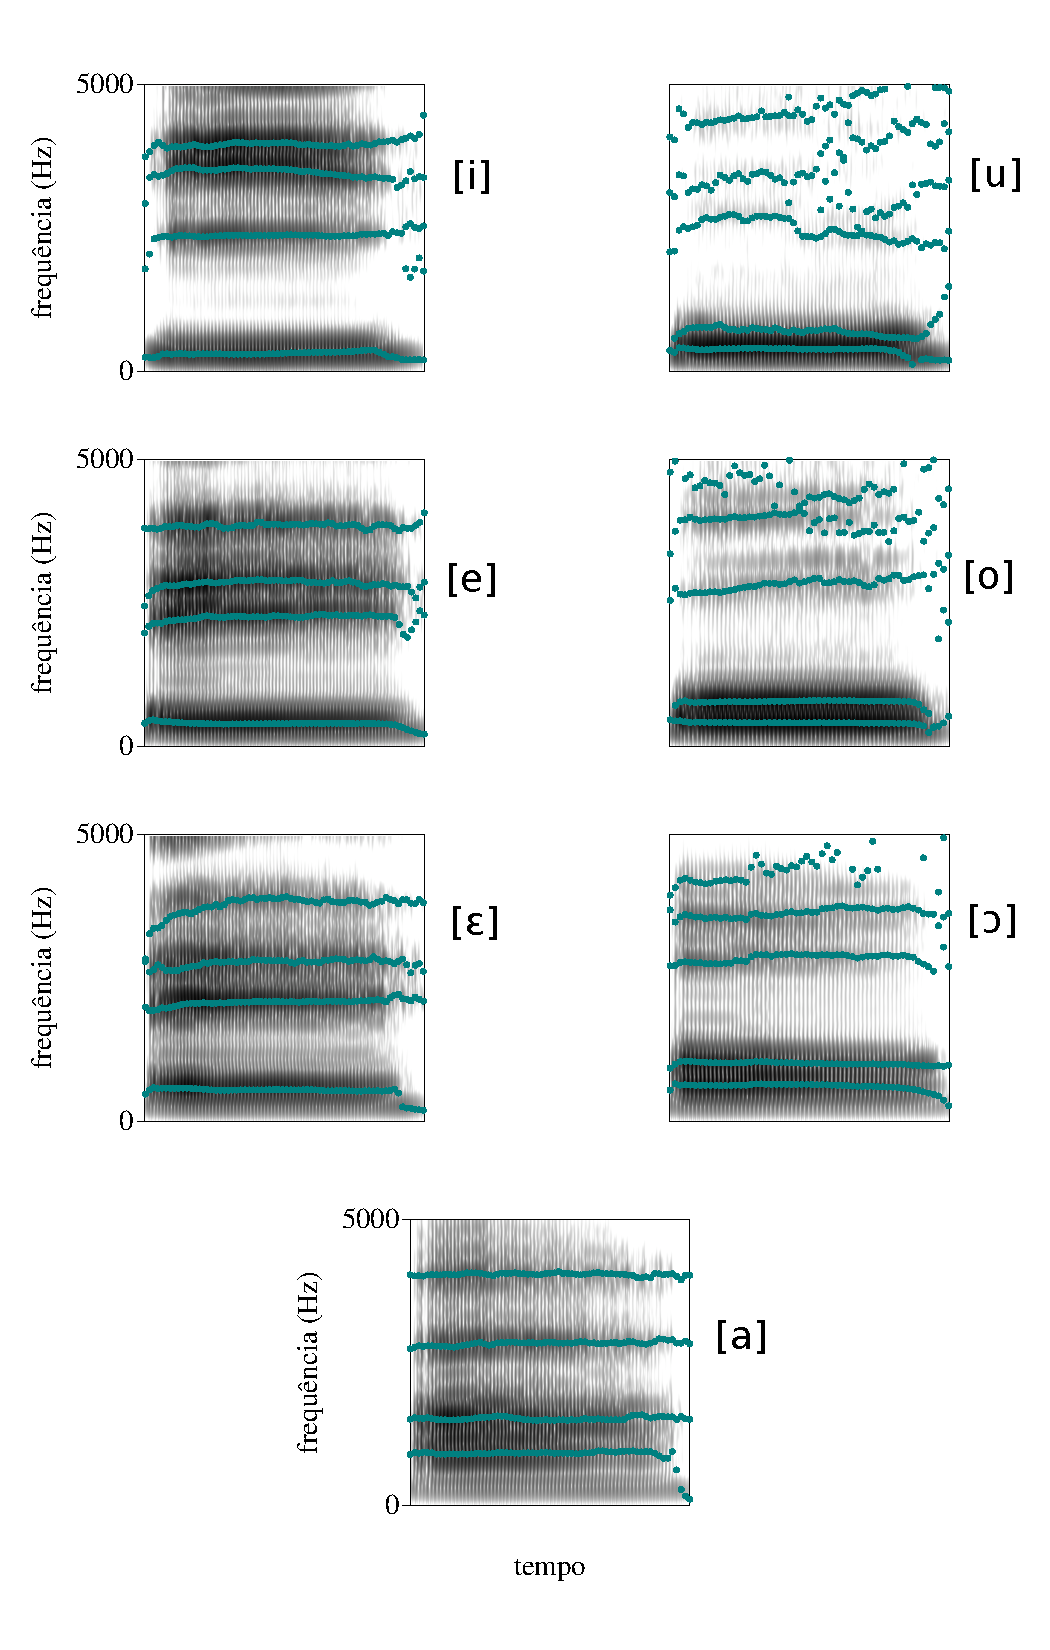
\includegraphics[width=0.73\textwidth]{Fig12.pdf}
 \caption{Espectrogramas com os formantes das sete vogais orais tensas do português.}
 \label{fig12}
  \source{Elaboração própria.}
\end{figure}
%%FIGURA 12 - Espectrogramas com os formantes das sete vogais orais tensas do português

Na Figura \ref{fig12}, os traçados dos formantes, em verde, foram sobrepostos aos espectrogramas. Os trechos em que foram traçados pontos dispersos em lugar de linhas correspondem a erros na medição dos formantes e são comuns nos formantes superiores, especialmente em vogais posteriores, e no início e fim das vogais. Além disso, note-se que os espectrogramas foram desenhados em gráficos de mesmo tamanho, mas as vogais apresentavam durações diferentes. Por essa razão, os valores do eixo do tempo foram omitidos, mas sem perda de informação, já que a imagem procurou enfatizar os formantes das vogais. 

O traçado dos formantes mostrado na Figura \ref{fig12} é gerado pelo Praat por meio da análise LPC (\textit{linear predictive coding}), técnica que permite estimar os picos das ressonâncias geradas pelo trato vocal a partir de um modelo físico de produção da fala. O Praat conta com comandos específicos para visualização e medição dos formantes. Para habilitar a visualização de formantes no espectrograma de um áudio, acesse \textit{Formant $\rightarrow$ Show Formants}. Após ativar essa opção, aparecerão pontos vermelhos formando um traçado para representar cada formante no espectrograma. Para extrair o valor de um formante, basta selecionar um intervalo de tempo contendo uma vogal e acessar \textit{Formant $\rightarrow$ Get X Formant} (com X podendo ser \textit{first}, \textit{second}, \textit{third} ou \textit{fourth}). Para além dos quatro primeiros é necessário selecionar \textit{Get Formant} e especificar o formante desejado na nova janela que aparecerá. Os valores dos quatro primeiros formantes ao longo de um intervalo de tempo podem ser extraídos juntos em \textit{Formant $\rightarrow$ Formant Listing}. Na medição de formantes, é importante estabelecer previamente um critério de medição, que deve incluir uma definição do(s) ponto(s) de medição (por exemplo, no centro do intervalo) e do número de medições (uma ou várias). A análise de formantes pode ser usada para caracterizar algumas consoantes (oclusivas e fricativas quanto a ponto de articulação, além de nasais, laterais, retroflexas), mas é frequentemente empregada na avaliação da qualidade vocálica. No caso da avaliação de vogais, as fronteiras inicial e final da vogal devem ser evitadas, pois são regiões cujas características acústicas refletem a transição articulatória com os sons adjacentes, dando-se preferência à região central da vogal, ou de maior estabilidade.  

Por vezes, acontece de os formantes identificados pelo Praat pelos círculos vermelhos não corresponderem às faixas escuras horizontais do espectrograma, como os pontos dispersos na Figura \ref{fig12}. Esse problema pode ser resolvido ao se ajustar parâmetros em \textit{Formant $\rightarrow$ Formant Settings}. Ao selecionar essa opção, será aberta uma janela com as configurações padrão. Pode-se tentar ajustar o número de formantes que o Praat deve encontrar no intervalo, que por padrão é 5, para um número maior ou menor. Pode-se também ajustar a frequência máxima do intervalo (\textit{formant ceiling}). Em geral, espera-se encontrar cinco formantes em um intervalo de cerca de 5000 Hz, o que equivale, em média, a um formante a cada 1000 Hz. Por padrão, as configurações dos parâmetros de identificação de formantes no Praat são cinco formantes em um intervalo que vai até 5500 Hz, o que é considerado adequado para mulheres. No caso dos homens, que apresentam, em média, trato vocal menor que as mulheres, o valor de 5500 Hz pode ser abaixado para 5000 Hz para se obter melhores medidas. Os parâmetros utilizados para identificação dos formantes dependem não só do falante (e seu trato vocal), mas também dos sons específicos: vogais anteriores podem exigir um intervalo superior a 5500 ou 5000 Hz, para que, por exemplo, formantes espúrios não sejam achados entre F1 e F2; por outro lado, os formantes de vogais posteriores podem muitas vezes ser melhor identificados ao se aumentar o número de formantes no intervalo, de forma a não ocasionar a identificação de um único formante no lugar de F1 e F2 (que em vogais posteriores são naturalmente próximos, dificultando a sua correta identificação). Pode ser conveniente adotar algum procedimento de ajuste desses parâmetros por falante e por vogal, seja de forma manual ou automatizada, p. ex. o procedimento de otimização descrito por \textcite[s.~2E]{escudero_2009}.

\subsection{Espectrogramas}\label{sec-espectrogramas}
Na geração de espectrogramas, é necessário usar uma janela (um trecho de tamanho constante) na qual é realizada a análise espectral de decomposição de frequências. Há dois modelos de espectrograma, de acordo com o tamanho da janela utilizada: o de banda larga e o de banda estreita. No espectrograma de banda larga é usada uma janela (em geral, com cerca de 0,005 s) menor que a janela do espectrograma de banda estreita (em geral, com cerca de 0,025 s). Como consequência, a análise em banda larga evidencia frequências em menor detalhamento (ou em menor resolução): não é capaz de mostrar os harmônicos, que são picos em regiões de frequência bem localizados, mas apenas picos mais amplos, como os formantes. Quando a janela utilizada é aumentada, é possível estimar em mais detalhamento as frequências componentes, de forma que a análise em banda estreita evidencia os picos mais localizados, correspondentes aos harmônicos, enquanto picos mais amplos, como os formantes, deixam de ser evidentes. Esses valores podem ser ajustados no Praat em \textit{Spectrum $\rightarrow$ Spectrogram settings}, em \textit{window length}. Por padrão, as configurações de espectrograma do Praat são adequadas para a visualização de formantes, sendo usada uma janela de 0,005 s, correspondente ao modelo de banda larga. A Figura \ref{fig13} ilustra espectrogramas em banda larga e em banda estreita para o mesmo áudio, correspondente a uma vogal [\textipa{E}].

\begin{figure}[htbp]
 \centering
 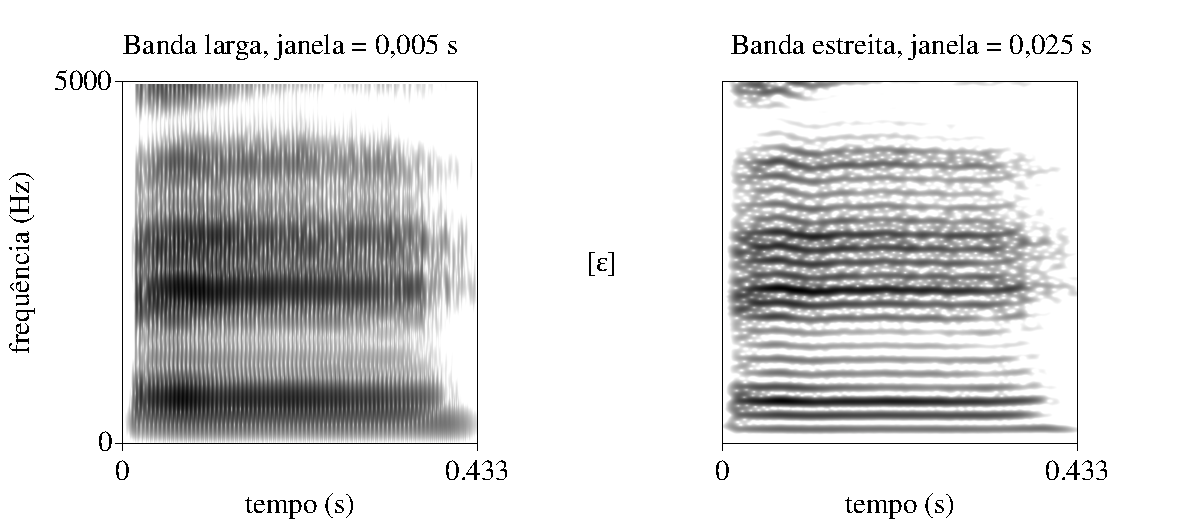
\includegraphics[width=1\textwidth]{Fig13.pdf}
 \caption{Exemplo de espectrograma de banda larga e banda estreita.}
 \label{fig13}
  \source{Elaboração própria.}
\end{figure}
%%Figura 13 - Exemplo de espectrograma de banda larga e banda estreita 

A Figura \ref{fig13}, à esquerda, mostra o espectrograma gerado com janela de 0,005 s, correspondente à configuração de banda larga. A resolução em frequência é baixa, de forma que as faixas horizontais correspondem aos formantes da vogal. À direita, é mostrado o espectrograma gerado com janela de 0,025 s, correspondente à configuração de banda estreita, para o mesmo trecho de áudio. A resolução em frequência é alta, de forma que as faixas horizontais correspondem aos harmônicos da vogal.

Outras opções que aparecem em \textit{Spectrogram settings} são o \textit{view range} e o \textit{dynamic range}. O \textit{view range} (intervalo de visualização) determina o valor mínimo e máximo que serão usados no eixo vertical de um espectrograma. Para análise de vogais, o valor máximo padrão de 5.000 Hz é adequado, pois nele estão contidos os três primeiros formantes. Para análise de consoantes, pode ser necessário aumentar o intervalo de visualização, possivelmente para 10.000 Hz, como será destacado na próxima seção. Por outro lado, o \textit{dynamic range} (intervalo dinâmico) diz respeito à diferença entre os valores de máxima e mínima potência no intervalo exibido. Por padrão, esse parâmetro no Praat tem o valor de 70 dB, mas deve ser ajustado de acordo com o nível de ruído presente no áudio. Muitas vezes, valores menores, como 60 dB ou 50 dB são mais convenientes para identificação dos padrões no espectrograma. No caso de arquivos de áudio ruidosos, pode ser abaixado para 40 dB ou 30 dB. Destaca-se que essas configurações em \textit{Spectrogram settings} não afetam o arquivo de áudio em análise, mas somente a visualização de seu espectrograma.

\subsection{Medição da duração}\label{sec-duracao}
Para extrair a duração de uma vogal (ou de qualquer outro segmento) é necessário primeiro selecionar o intervalo de tempo dentro do qual a vogal ocorre fazendo o uso de um critério de segmentação. Delimitada a vogal, é possível extrair a duração acessando \textit{Query $\rightarrow$ Get Selection Length}, que abrirá uma nova janela com medida. A duração de uma seleção também pode ser inspecionada rapidamente na barra superior cinza imediatamente acima da forma de onda. O Praat usa apenas o segundo como unidade de medida para a duração e outras informações temporais. Por fim, alertamos que, especialmente em medidas de duração, é crucial contar com critérios de segmentação bem estabelecidos e seguidos sistematicamente, pois afetam diretamente a grandeza que está sendo medida. Além disso, como já mencionado anteriormente, quanto menor a unidade avaliada, mais precisa deve ser a segmentação. 

\section{Análise acústica das consoantes}\label{sec-consoantes}
As consoantes formam um grupo de sons foneticamente distintos entre si, especialmente em decorrência dos diferentes modos de articulação. Nesta seção, iremos apresentar algumas propriedades acústicas das consoantes e como tais propriedades podem ser associadas a características articulatórias, nos concentrando nas oclusivas e fricativas. Também serão abordados métodos de medição mais frequentemente utilizados para avaliação acústica desses sons.

Articulatoriamente, as consoantes são descritas de acordo com a obstrução que as caracteriza. São classificadas quanto ao seu ponto e seu modo de articulação, além da presença ou ausência de vozeamento. É possível associar diferenças articulatórias a características acústicas presentes nas ondas sonoras das consoantes. 

As oclusivas correspondem articulatoriamente a uma sequência de ações: fechamento completo do trato vocal, seguido de soltura ou liberação do fechamento, de forma abrupta. Se houver uma vogal depois da oclusiva, haverá uma transição articulatória entre a configuração do trato na consoante e a configuração que será usada na vogal. É possível também que ocorra após a soltura uma aspiração. Acusticamente, identificamos como característica do fechamento uma redução drástica na amplitude do sinal no gráfico da forma de onda e, no espectrograma, uma faixa branca, que demonstra a escassez de energia acústica em todas as faixas do espectro, com exceção da região da frequência fundamental, caso seja uma vozeada. A soltura corresponde acusticamente a um transiente, isto é, a uma variação rápida na amplitude na forma de onda e, no espectrograma, a uma faixa escura, indicando uma elevada densidade de energia acústica, percorrendo boa parte das frequências. A aspiração, quando presente, corresponde a um sinal aperiódico contínuo semelhante ao ruído fricativo.

As fricativas são consoantes em que a obstrução representa um forte estreitamento à passagem da corrente de ar, sem que haja, contudo, um bloqueio completo, como nas oclusivas. Nesse tipo de obstrução, é estabelecido um padrão de fricção entre os articuladores, que tem como consequência, acusticamente, a produção de uma onda sonora aperiódica contínua. No caso de fricativas vozeadas, as aperiodicidades são sobrepostas à periodicidade do vozeamento. As fricativas compartilham com as oclusivas alguns métodos de avaliação acústica. 

O valor de F2 e F3 na transição entre uma oclusiva e uma vogal adjacente pode ser usado para avaliação do ponto de articulação da oclusiva. A medição dos formantes é realizada tal como descrito na seção 5, para análise de vogais, com exceção do ponto de medição: neste caso, busca-se justamente o ponto de transição da vogal com a consoante (ao invés de uma porção estável, no meio da vogal, no caso da avaliação da qualidade vocálica). O valor de F2 e F3 na transição depende da qualidade da vogal, devendo-se comparar as medições realizadas em uma mesma vogal. De modo geral, consoantes bilabiais apresentam F2 mais baixo do que alveolares; alveolares, valor de F2 mais baixo do que velares. O valor de F3 também pode ser usado para caracterização do ponto, mas não será abordado aqui. A Figura \ref{fig14} mostra espectrogramas de três consoantes oclusivas intervocálicas ([p], [t] e [k]), destacando com uma seta azul os pontos de medição de F2 na vogal seguinte e seus respectivos valores, que crescem acompanhando a posteriorização da oclusão. Os intervalos dos eixos horizontais foram omitidos por não serem relevantes para a medição em questão. Os formantes na transição com uma vogal também são afetados pelo ponto de articulação das fricativas, mas a avaliação espectral é mais frequentemente empregada na avaliação do ponto desse grupo de sons. 

\begin{figure}[H]
 \centering
 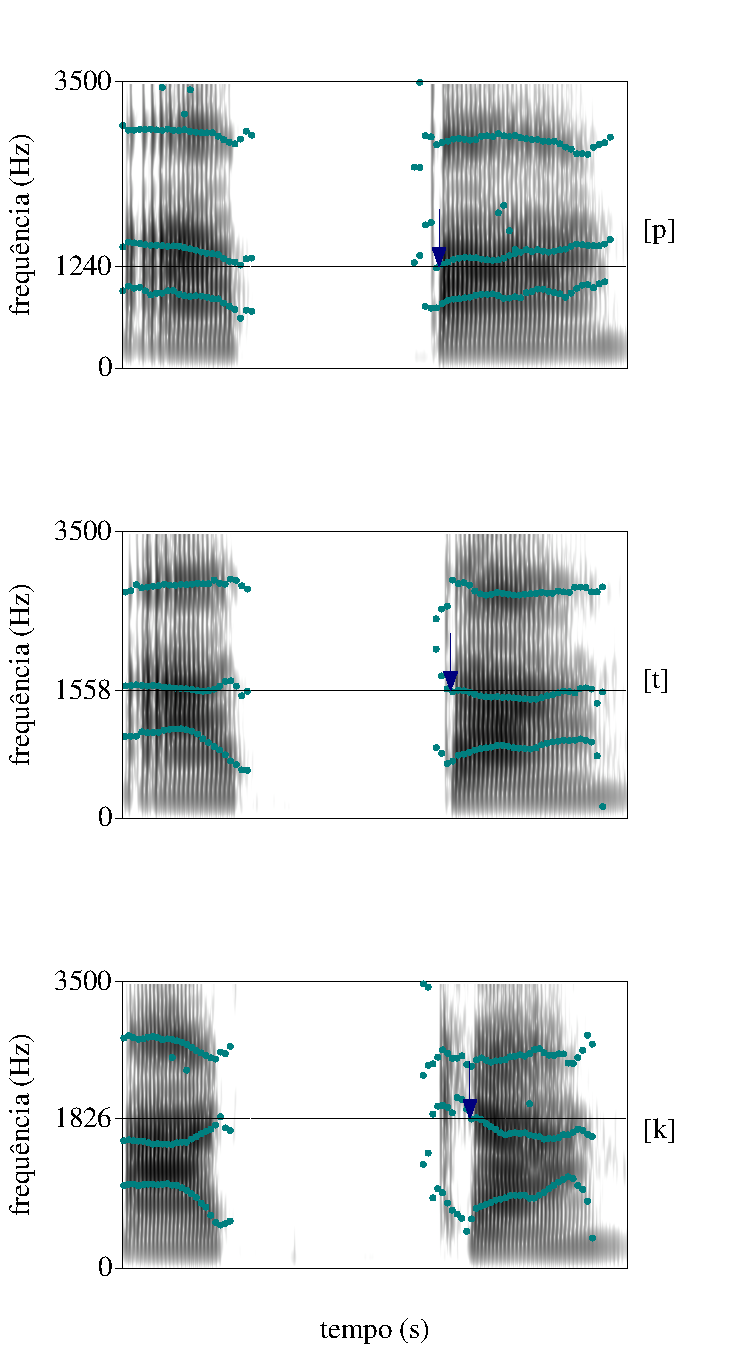
\includegraphics[width=0.7\textwidth]{Fig14.pdf}
 \caption{Espectrogramas de oclusivas intervocálicas e medição do F2 na transição.}
 \label{fig14}
  \source{Elaboração própria.}
\end{figure}
%%FIGURA 14 - Espectrogramas de oclusivas intervocálicas e medição do F2 na transição

Outras medidas acústicas podem ser usadas para caracterizar ponto de articulação de oclusivas e fricativas, com destaque para medidas relacionadas a características espectrais, mas não serão abordadas neste material, por limitação de extensão do texto.

O vozeamento das consoantes oclusivas e fricativas pode ser avaliado acusticamente, na forma de onda, pelas oscilações periódicas aproximadamente senoidais, no trecho que corresponde ao fechamento. No espectrograma, o vozeamento pode ser identificado pela presença de uma faixa escura na região de frequência correspondente à frequência fundamental da voz. Esta faixa é chamada de barra de vozeamento. A Figura \ref{fig15} mostra a forma de onda e o espectrograma de consoantes oclusivas e fricativas não vozeadas, acima, e vozeadas, abaixo, em contexto intervocálico. Um retângulo azul identifica a barra de vozeamento nas vozeadas, ausente nas não vozeadas.

\begin{figure}[H]
 \centering
 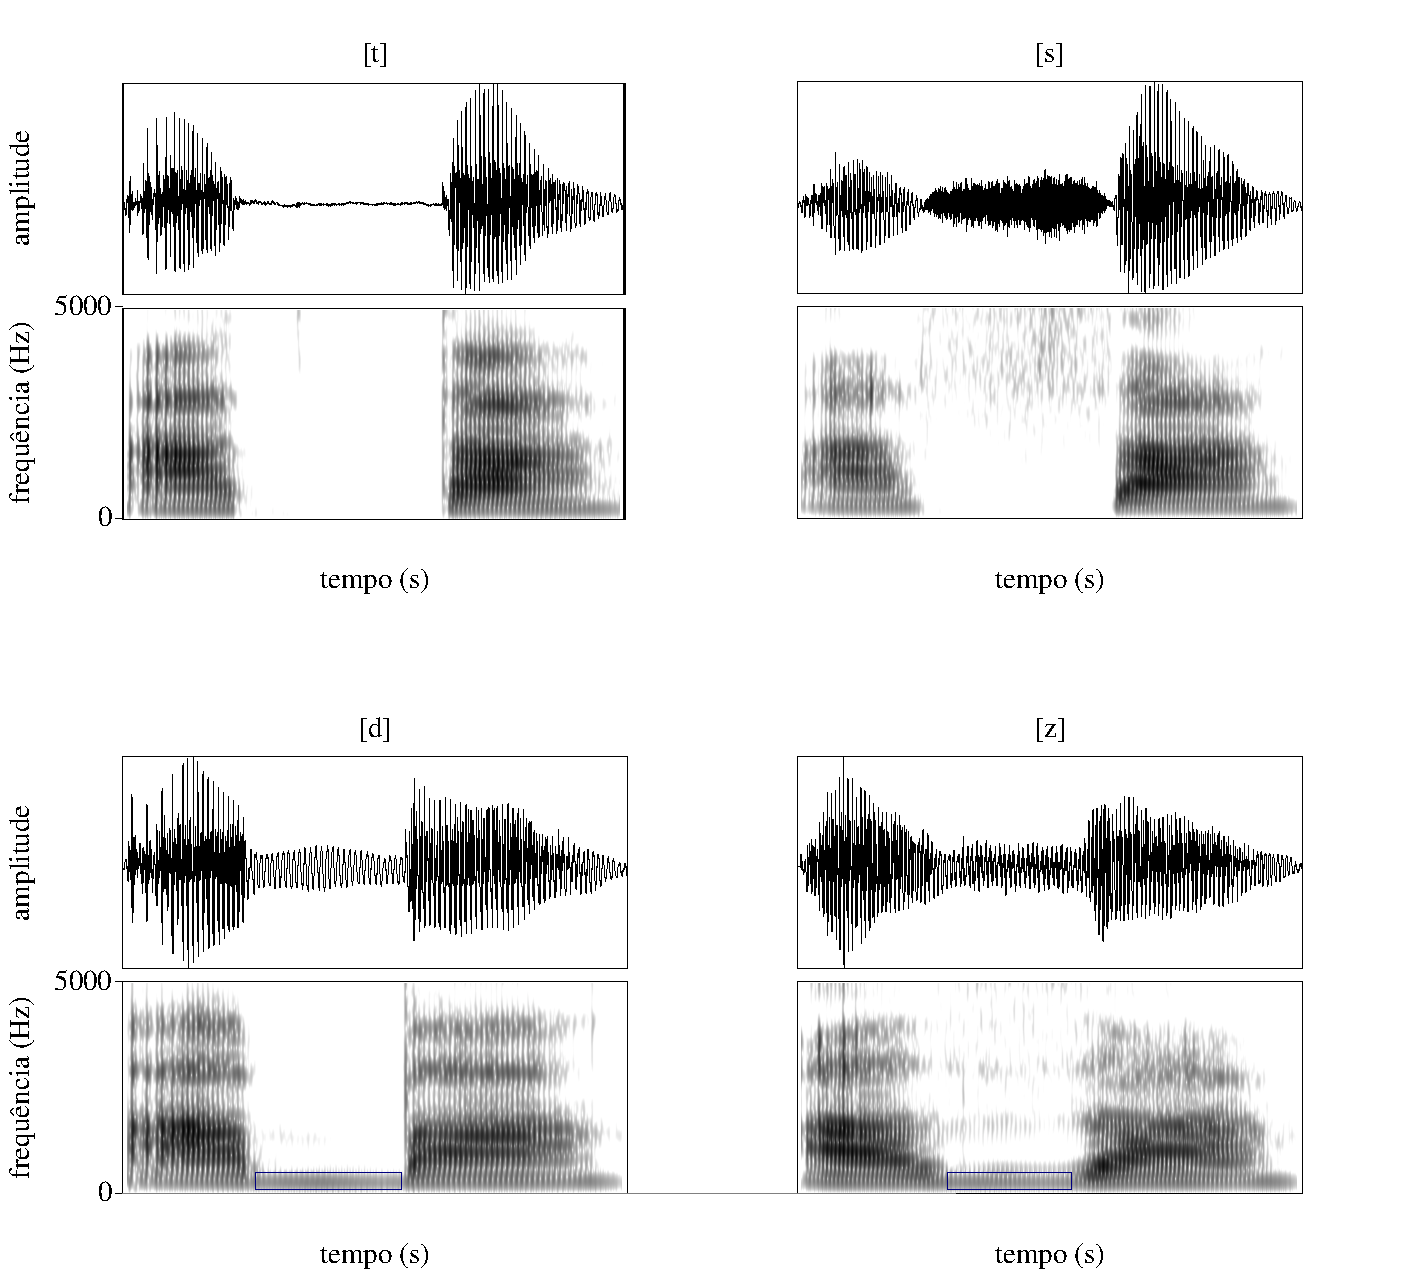
\includegraphics[width=0.9\textwidth]{Fig15.pdf}
 \caption{Forma de onda e espectrograma de consoantes com indicação da barra de vozeamento.}
 \label{fig15}
  \source{Elaboração própria.}
\end{figure}
%%FIGURA 15 - Forma de onda e espectrograma de consoantes com indicação da barra de vozeamento

Nas oclusivas, a presença de aspiração após a soltura pode ser avaliada acusticamente por uma medida chamada VOT (\textit{voice onset time}, ou tempo para início do vozeamento). Essa medida permite não apenas quantificar a aspiração, mas estabelecer uma oposição entre oclusivas vozeadas, oclusivas não vozeadas não aspiradas e oclusivas não vozeadas aspiradas. É especialmente útil em línguas que utilizam essa diferenciação acústica de forma contrastiva. O VOT é uma medida de duração realizada em oclusiva seguida de vogal, a partir de dois pontos de referência: o ponto de soltura (S) da oclusiva e o ponto em que se inicia o vozeamento (V) (que pode ser na própria consoante, no caso se vozeadas, ou na vogal, no caso de não vozeadas). O VOT é obtido pela operação VOT = V -- S. Vozeadas apresentam VOT negativo, pois o vozeamento ocorre antes da soltura, ainda durante o fechamento. Não vozeadas que não são aspiradas apresentam VOT próximo de zero, podendo ser ligeiramente positivo. Aspiradas apresentam VOT positivo superior ao das não aspiradas, podendo ser da ordem de 50 a 120 ms (mas esse valor depende da língua). A Figura \ref{fig16} mostra a medição de VOT para três oclusivas do português: [t], [g] e [k]. Os eixos horizontais não apresentam o mesmo intervalo. Seus valores foram omitidos por economia, mas os pontos temporais importantes foram assinalados. Ainda que no português a aspiração das oclusivas não tenha função contrastiva, observa-se que a velar não vozeada apresenta certo grau de aspiração, como é comum também em outras línguas.  

\begin{figure}[H]
 \centering
 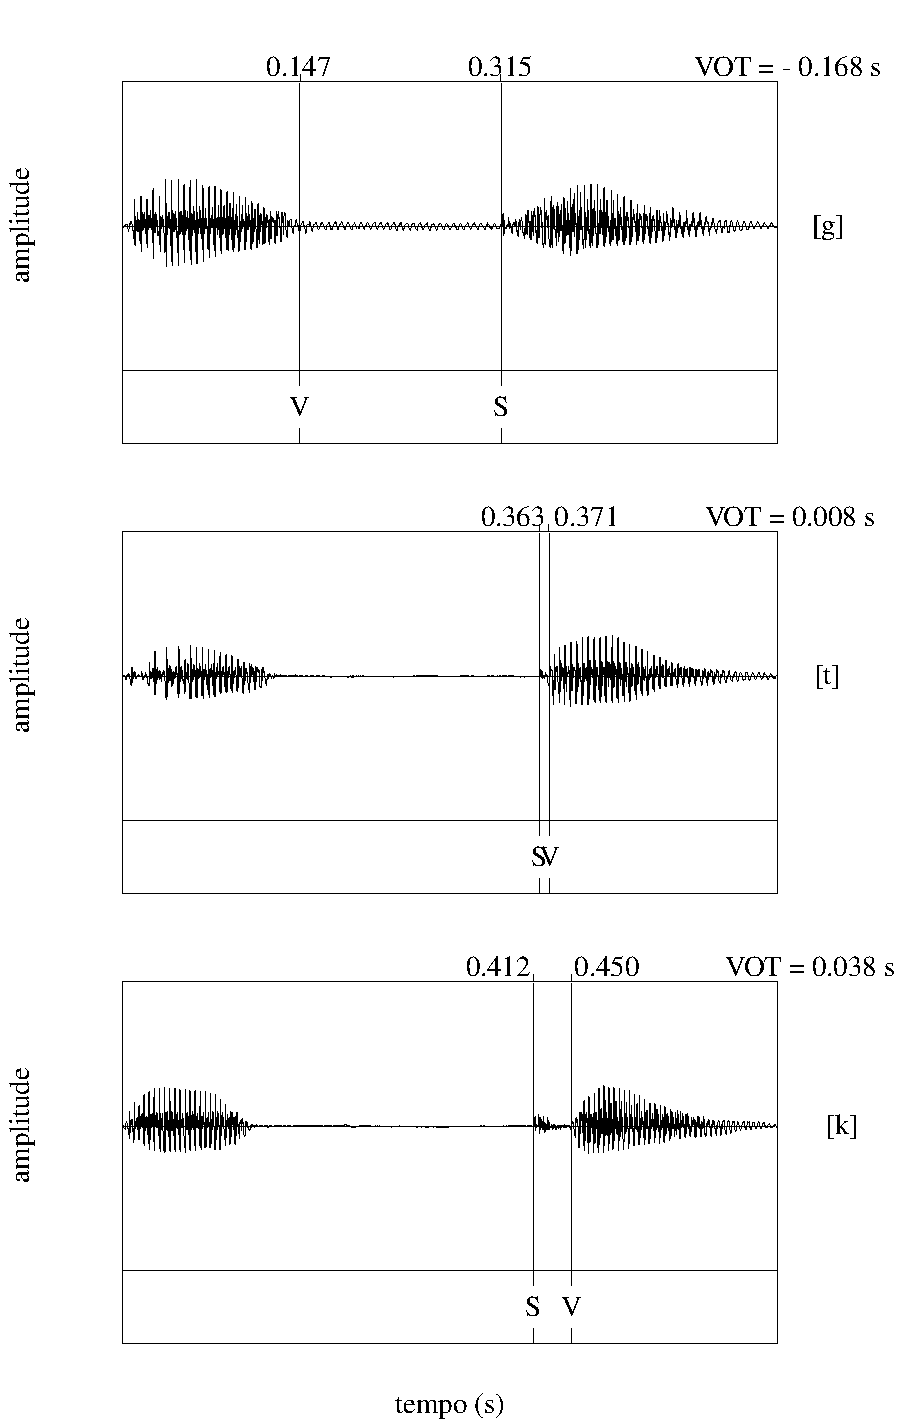
\includegraphics[width=0.65\textwidth]{Fig16.pdf}
 \caption{Forma de onda de oclusivas com medição de VOT.}
 \label{fig16}
  \source{Elaboração própria.}
\end{figure}
%%FIGURA 16 - Forma de onda de oclusivas com medição de VOT

\section{Análise acústica prosódica}\label{sec-prosodia}
Nesta seção, trataremos brevemente de métodos de análise acústica prosódica, suas especificidades e alguns conceitos elementares. Serão enfocados especialmente dois temas da análise prosódica, a entoação e a organização temporal da fala, que permitem explorar análises no domínio do tempo e no domínio da frequência, respectivamente.

\subsection{Entoação e curva melódica}\label{sec-entoacao}
A entoação pode ser definida como variações da frequência fundamental da fala ao longo de grupos de palavras, associadas a propriedades sintáticas e pragmáticas. Estabelece na linguagem as funções de segmentação e proeminência, funções que podem ser exercidas também por outros elementos prosódicos, por exemplo, ritmo e elementos da organização temporal da fala, como pausas e alongamentos. Além dessas funções, permite ou está envolvida na expressão de atitudes e na expressão de emoções.

A variação frequência fundamental pode ser observada em espectrograma, ao se utilizar a configuração de banda estreita, que consiste em aumentar a janela em relação à janela do espectrograma padrão, de banda larga, padrão no Praat e o adequado para a análise de formantes, em \textit{Spectrum $\rightarrow$ Spectrogram Settings}, com \textit{window length} = 0.025, como mencionado na seção sobre vogais. O aumento da janela para 0,025 s diminui a resolução temporal mas leva a um aumento da resolução em frequência, o que permite a visualização da estrutura harmônica das ondas sonoras, no espectrograma de banda estreita.

O traçado da variação da frequência fundamental ao longo de enunciados corresponde ao que se chama de curva entoacional ou curva melódica. Sua avaliação implica em monitorar os valores de F0 ao longo do tempo. O Praat apresenta o recurso de rastreamento de F0 (\textit{pitch tracking}), que pode ser utilizado para analisar a curva entoacional. Para habilitar o recurso, deve-se selecionar \textit{Pitch $\rightarrow$ Show Pitch}. Após essa seleção, aparecerá uma linha em azul mostrando a variação da curva de F0 ao longo da gravação, por padrão, sobreposta ao espectrograma. Observe que essa curva em azul corresponde a um novo eixo vertical de frequência, que estará localizado à direita e tem extensão diferente do eixo vertical de frequências da esquerda, que se refere ao espectrograma. A curva de F0 gerada pelo programa é um gráfico independente do espectrograma (experimente suprimir o espectrograma, com \textit{Spectrum $\rightarrow$ Show Spectrum} (desabilitado)). Pode ser transformada em um objeto independente, que aparecerá na janela de objetos e pode ser submetido a medições e manipulação, ao se selecionar \textit{Pitch $\rightarrow$ Extract visible pitch contour}. Opções relevantes para o objeto de tipo \textit{pitch} serão apresentadas no menu dinâmico da janela de objetos. A Figura \ref{fig17} apresenta dois exemplos de enunciados, contendo a expressão ``Fomos convidados para a festa'', em uma declaração (acima) e em uma afirmação (abaixo). 

A curva de F0 (em azul, relativa ao eixo direito) coincide com as curvas visualizadas no espectrograma (que mostra a estrutura harmônica, referenciada ao eixo esquerdo). A trajetória das curvas das duas sentenças são distintas, especialmente na porção final, em que a interrogativa apresenta uma elevação. Há algumas irregularidades locais, que decorrem principalmente de mecanismos aerodinâmicos envolvidos na produção de consoantes, e que não são do interesse para a análise entoacional.

Caso a curva gerada apresente trechos inadequados (indicando vozeamento onde não há, ou falhando em trechos vozeados) ou ainda descontinuidades (subitamente sendo dobrada ou reduzida pela metade), é necessário fazer ajustes no rastreador de F0. Melhores resultados podem ser obtidos ao se ajustar, em \textit{Pitch $\rightarrow$ Pitch settings}, os valores de \textit{Pitch range} a um intervalo um pouco mais amplo que o intervalo de F0 do falante em análise, determinado a partir do espectrograma de banda estreita ou por \textit{Pitch → Get minimum Pitch} e \textit{Pitch $\rightarrow$ Get maximum pitch}. Se a curva de F0 não estiver sendo exibida no áudio, em longos trechos ou de modo geral, tente aumentar, em \textit{Pitch $\rightarrow$ Advanced Pitch settings}, o valor de \textit{Silence threshold}. Caso a curva esteja inadequada em alguns trechos, experimente ajustar o valor de \textit{Voicing threshold}. No caso de descontinuidades na curva de F0, experimente aumentar o valor de \textit{Octave-jump cost}.

\begin{figure}[H]
 \centering
 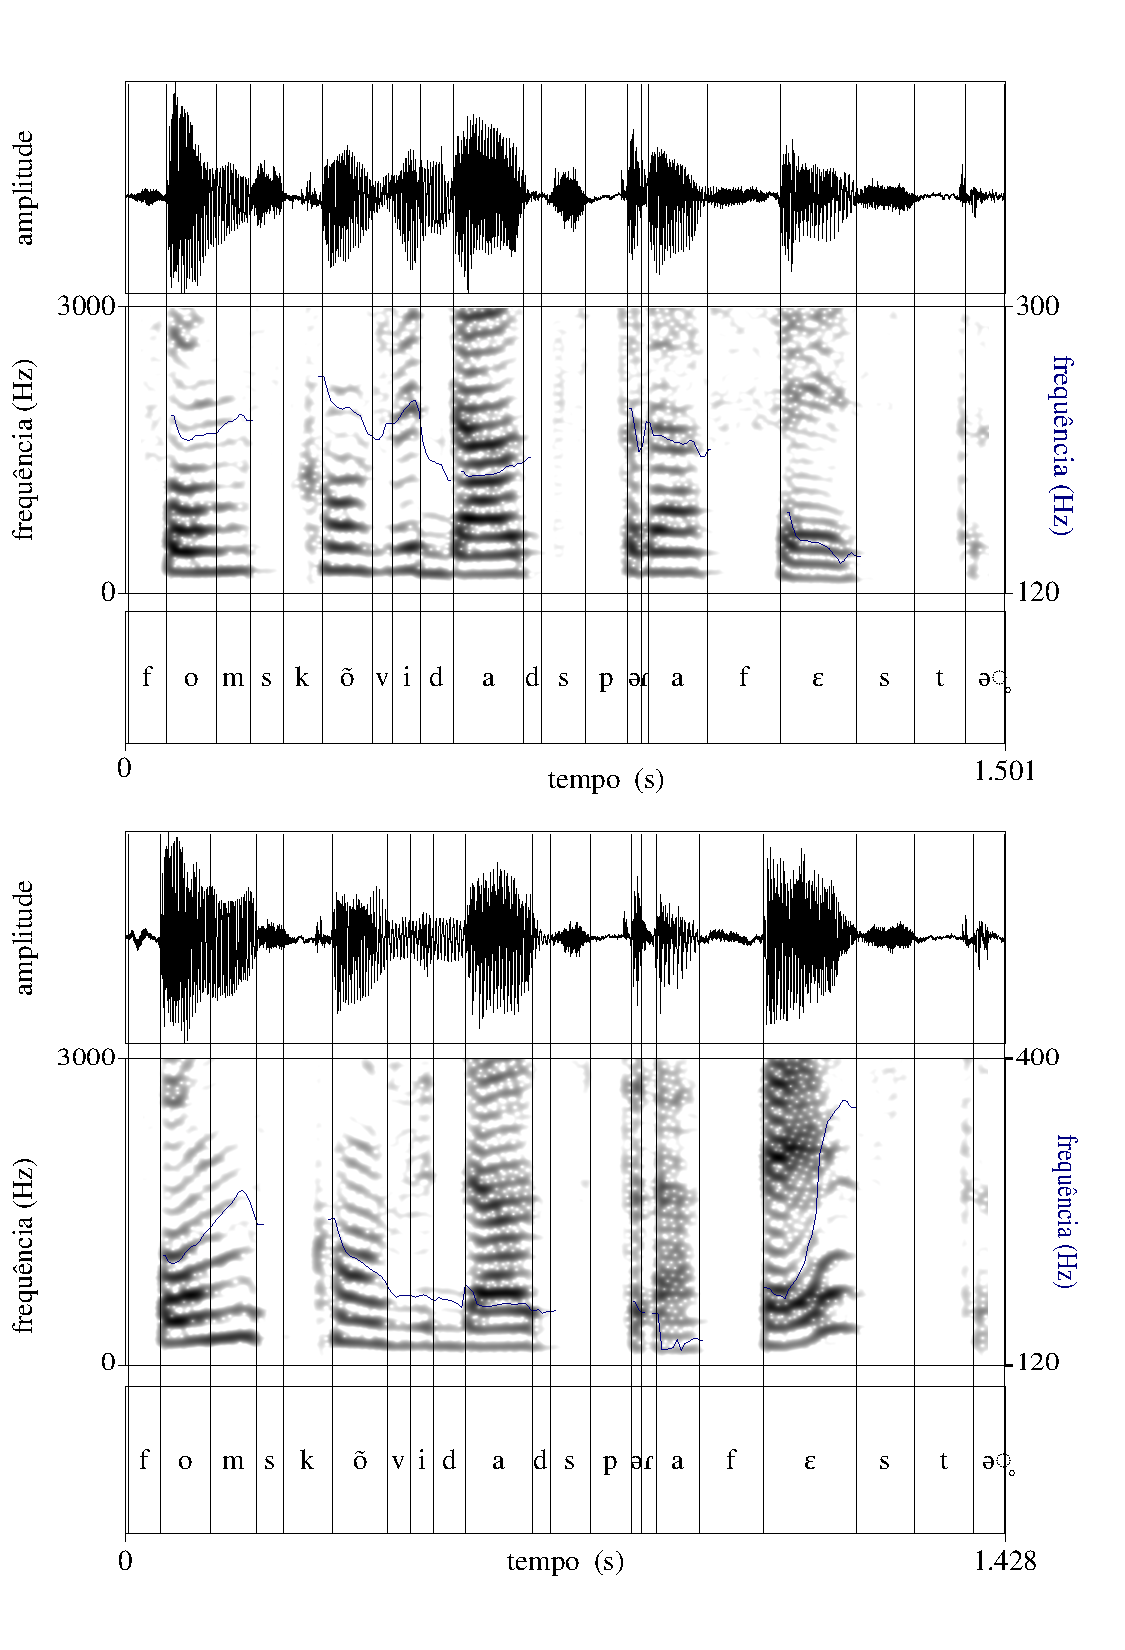
\includegraphics[width=1\textwidth]{Fig17.pdf}
 \caption{Forma de onda, espectrograma de banda estreita e curva de F0 de duas sentenças com entoações distintas.}
 \label{fig17}
  \source{Elaboração própria.}
\end{figure}
%%FIGURA 17 - Forma de onda, espectrograma de banda estreita e curva de F0 de duas sentenças com entoações distintas

\subsection{Organização temporal da fala}\label{sec-organizacao}
A organização temporal da fala se refere a como organizamos durações de segmentos, sílabas e pausas ao longo dos enunciados. Duas medidas tradicionais são empregadas para caracterização da organização temporal da fala: taxa de elocução e de articulação. A taxa de elocução corresponde ao número de unidades linguísticas por unidade de tempo (palavras por minuto, sílabas por segundo ou fones por segundo), enquanto a taxa de articulação consiste na divisão do número de sílabas pelo tempo de articulação, excluindo desse tempo a duração das pausas. Para medir as taxas de elocução e articulação é recomendado que todas as sílabas (ou fones, ou palavras) sejam adequadamente delimitadas e etiquetadas com algum texto no rótulo (cf. \Cref{sec-segmentacao}). A taxa de elocução pode ser então obtida por meio de \textit{scripts} ou pelo seguinte procedimento: na janela de visualização e edição do TextGrid com áudio, selecione \textit{File $\rightarrow$ Preferences $\rightarrow$ Show number of... non-empty intervals or points}. Ao selecionar essa opção, o número que aparecerá entre parênteses abaixo do nome da camada, na janela de visualização, corresponderá ao número de intervalos da camada que contém algum preenchimento. Considerando que esses intervalos preenchidos correspondem exatamente às unidades usadas para obter a taxa de elocução, seu cálculo pode ser feito dividindo-se a duração total do enunciado pelo número de intervalos preenchidos. A duração total do intervalo pode ser obtida em \textit{Total Duration} na faixa cinza na parte mais inferior da janela, se o início e o fim do arquivo corresponderem ao início e fim da elocução. Caso existam trechos silenciosos no início e no fim da gravação, o trecho exato do enunciado pode ser selecionado e a duração da seleção, que aparece na faixa cinza logo acima da forma de onda, utilizada para obter a duração total do enunciado. A taxa de articulação exige a eliminação das durações correspondentes às pausas e pode ser feita preferencialmente por \textit{script}, após a identificação das pausas no TextGrid.

\section{Considerações finais}\label{sec-consideracoes}
Os diferentes sons da fala envolvem padrões acústicos específicos, que podem ser identificados e mensurados com ferramentas gráficas. Nos primórdios dos estudos da fala, essas ferramentas eram grandes equipamentos analógicos e especializados (como o espectrógrafo do som desenvolvido nos Laboratórios Bell na década de 1940'). Posteriormente, com a ampla difusão dos microcomputadores, a representação gráfica dos sons passou a ser realizada por programas computacionais. O Praat é um programa de análise acústica especializado que revolucionou o estudo da fala no mundo todo, por sua gratuidade, sua robustez e sua transparência, permitindo o acesso amplo e democrático a recursos técnicos de qualidade.   

Neste texto, procuramos apresentar como tarefas fundamentais da análise acústica podem ser realizadas no \textit{software}, contribuindo para a compreensão dos métodos de avaliação da fala e incentivando mais pesquisadores a utilizarem o programa em suas análises. Em conformidade com os objetivos propostos, foram apresentados os procedimentos elementares para inspeção gráfica e medição de vogais e consoantes, assim como a avaliação da organização temporal da fala e curva entoacional. As dimensões deste trabalho, contudo, restringiram os procedimentos aos métodos mais básicos, cabendo a estudos futuros detalhar procedimentos mais avançados de análise acústica e como podem ser realizados com recursos do Praat.


\printbibliography\label{sec-bib}
% if the text is not in Portuguese, it might be necessary to use the code below instead to print the correct ABNT abbreviations [s.n.], [s.l.]
%\begin{portuguese}
%\printbibliography[title={Bibliography}]
%\end{portuguese}


%full list: conceptualization,datacuration,formalanalysis,funding,investigation,methodology,projadm,resources,software,supervision,validation,visualization,writing,review
\begin{contributors}[sec-contributors]
\authorcontribution{Maria Mendes Cantoni}[conceptualization,projadm,formalanalysis,resources,supervision,writing,review]
\authorcontribution{Bárbara de Oliveira Godinho}[conceptualization,writing,review]
\authorcontribution{Henrique Mancini Nevado}[conceptualization,writing,review]
\end{contributors}

\end{document}

